\documentclass[twoside]{book}

% Packages required by doxygen
\usepackage{fixltx2e}
\usepackage{calc}
\usepackage{doxygen}
\usepackage[export]{adjustbox} % also loads graphicx
\usepackage{graphicx}
\usepackage[utf8]{inputenc}
\usepackage{makeidx}
\usepackage{multicol}
\usepackage{multirow}
\PassOptionsToPackage{warn}{textcomp}
\usepackage{textcomp}
\usepackage[nointegrals]{wasysym}
\usepackage[table]{xcolor}

% NLS support packages
\usepackage[french]{babel}

% Font selection
\usepackage[T1]{fontenc}
\usepackage[scaled=.90]{helvet}
\usepackage{courier}
\usepackage{amssymb}
\usepackage{sectsty}
\renewcommand{\familydefault}{\sfdefault}
\allsectionsfont{%
  \fontseries{bc}\selectfont%
  \color{darkgray}%
}
\renewcommand{\DoxyLabelFont}{%
  \fontseries{bc}\selectfont%
  \color{darkgray}%
}
\newcommand{\+}{\discretionary{\mbox{\scriptsize$\hookleftarrow$}}{}{}}

% Page & text layout
\usepackage{geometry}
\geometry{%
  a4paper,%
  top=2.5cm,%
  bottom=2.5cm,%
  left=2.5cm,%
  right=2.5cm%
}
\tolerance=750
\hfuzz=15pt
\hbadness=750
\setlength{\emergencystretch}{15pt}
\setlength{\parindent}{0cm}
\setlength{\parskip}{3ex plus 2ex minus 2ex}
\makeatletter
\renewcommand{\paragraph}{%
  \@startsection{paragraph}{4}{0ex}{-1.0ex}{1.0ex}{%
    \normalfont\normalsize\bfseries\SS@parafont%
  }%
}
\renewcommand{\subparagraph}{%
  \@startsection{subparagraph}{5}{0ex}{-1.0ex}{1.0ex}{%
    \normalfont\normalsize\bfseries\SS@subparafont%
  }%
}
\makeatother

% Headers & footers
\usepackage{fancyhdr}
\pagestyle{fancyplain}
\fancyhead[LE]{\fancyplain{}{\bfseries\thepage}}
\fancyhead[CE]{\fancyplain{}{}}
\fancyhead[RE]{\fancyplain{}{\bfseries\leftmark}}
\fancyhead[LO]{\fancyplain{}{\bfseries\rightmark}}
\fancyhead[CO]{\fancyplain{}{}}
\fancyhead[RO]{\fancyplain{}{\bfseries\thepage}}
\fancyfoot[LE]{\fancyplain{}{}}
\fancyfoot[CE]{\fancyplain{}{}}
\fancyfoot[RE]{\fancyplain{}{\bfseries\scriptsize Généré par Doxygen }}
\fancyfoot[LO]{\fancyplain{}{\bfseries\scriptsize Généré par Doxygen }}
\fancyfoot[CO]{\fancyplain{}{}}
\fancyfoot[RO]{\fancyplain{}{}}
\renewcommand{\footrulewidth}{0.4pt}
\renewcommand{\chaptermark}[1]{%
  \markboth{#1}{}%
}
\renewcommand{\sectionmark}[1]{%
  \markright{\thesection\ #1}%
}

% Indices & bibliography
\usepackage{natbib}
\usepackage[titles]{tocloft}
\setcounter{tocdepth}{3}
\setcounter{secnumdepth}{5}
\makeindex

% Hyperlinks (required, but should be loaded last)
\usepackage{ifpdf}
\ifpdf
  \usepackage[pdftex,pagebackref=true]{hyperref}
\else
  \usepackage[ps2pdf,pagebackref=true]{hyperref}
\fi
\hypersetup{%
  colorlinks=true,%
  linkcolor=blue,%
  citecolor=blue,%
  unicode%
}

% Custom commands
\newcommand{\clearemptydoublepage}{%
  \newpage{\pagestyle{empty}\cleardoublepage}%
}

\usepackage{caption}
\captionsetup{labelsep=space,justification=centering,font={bf},singlelinecheck=off,skip=4pt,position=top}

%===== C O N T E N T S =====

\begin{document}

% Titlepage & ToC
\hypersetup{pageanchor=false,
             bookmarksnumbered=true,
             pdfencoding=unicode
            }
\pagenumbering{roman}
\begin{titlepage}
\vspace*{7cm}
\begin{center}%
{\Large Model\+Dll }\\
\vspace*{1cm}
{\large Généré par Doxygen 1.8.11}\\
\end{center}
\end{titlepage}
\clearemptydoublepage
\tableofcontents
\clearemptydoublepage
\pagenumbering{arabic}
\hypersetup{pageanchor=true}

%--- Begin generated contents ---
\chapter{Index hiérarchique}
\section{Class Hierarchy}
This inheritance list is sorted roughly, but not completely, alphabetically\+:\begin{DoxyCompactList}
\item \contentsline{section}{My\+Domotik.\+Affichage}{\pageref{class_my_domotik_1_1_affichage}}{}
\item Application\begin{DoxyCompactList}
\item \contentsline{section}{My\+Domotik.\+App}{\pageref{class_my_domotik_1_1_app}}{}
\end{DoxyCompactList}
\item Page\begin{DoxyCompactList}
\item \contentsline{section}{My\+Domotik.\+Admin\+Page}{\pageref{class_my_domotik_1_1_admin_page}}{}
\item \contentsline{section}{My\+Domotik.\+Gestion\+Equipements}{\pageref{class_my_domotik_1_1_gestion_equipements}}{}
\item \contentsline{section}{My\+Domotik.\+Gestion\+Pieces}{\pageref{class_my_domotik_1_1_gestion_pieces}}{}
\item \contentsline{section}{My\+Domotik.\+Main\+Page}{\pageref{class_my_domotik_1_1_main_page}}{}
\item \contentsline{section}{My\+Domotik.\+Reglages\+Couleur}{\pageref{class_my_domotik_1_1_reglages_couleur}}{}
\item \contentsline{section}{My\+Domotik.\+Reglages\+Mode\+Selection}{\pageref{class_my_domotik_1_1_reglages_mode_selection}}{}
\item \contentsline{section}{My\+Domotik.\+Reglages\+Reseau}{\pageref{class_my_domotik_1_1_reglages_reseau}}{}
\item \contentsline{section}{My\+Domotik.\+Reglages\+Taille\+Icones}{\pageref{class_my_domotik_1_1_reglages_taille_icones}}{}
\end{DoxyCompactList}
\end{DoxyCompactList}

\chapter{Index des classes}
\section{Class List}
Here are the classes, structs, unions and interfaces with brief descriptions\+:\begin{DoxyCompactList}
\item\contentsline{section}{\hyperlink{classhappyhttp_1_1_connection}{happyhttp\+::\+Connection} }{\pageref{classhappyhttp_1_1_connection}}{}
\item\contentsline{section}{\hyperlink{class_requete}{Requete} \\*Classe a utilisée par la fonction void Dll\+Import \hyperlink{_requete_http_8h_aade1da46e511a08d213c2e2bc4533b43}{requete\+Http\+Kira(char$\ast$ s1, char$\ast$ s2)}; }{\pageref{class_requete}}{}
\item\contentsline{section}{\hyperlink{classhappyhttp_1_1_response}{happyhttp\+::\+Response} }{\pageref{classhappyhttp_1_1_response}}{}
\item\contentsline{section}{\hyperlink{classhappyhttp_1_1_wobbly}{happyhttp\+::\+Wobbly} }{\pageref{classhappyhttp_1_1_wobbly}}{}
\end{DoxyCompactList}

\chapter{Documentation des classes}
\hypertarget{class_e_p_1_1_core}{}\section{Référence de la classe EP\+:\+:Core}
\label{class_e_p_1_1_core}\index{E\+P\+::\+Core@{E\+P\+::\+Core}}


Le coeur de l\textquotesingle{}application, contient la liste des pièces, les paramètres de l\textquotesingle{}application ainsi que les méthodes pour gérer ceux-\/ci.  




{\ttfamily \#include $<$Core.\+h$>$}

\subsection*{Fonctions membres publiques}
\begin{DoxyCompactItemize}
\item 
\hyperlink{class_e_p_1_1_core_acfb517a0b01ff278283e940b184fcea4}{Core} (char $\ast$file)
\begin{DoxyCompactList}\small\item\em Le constructeur de Core.\+summary. \end{DoxyCompactList}\item 
\hyperlink{class_e_p_1_1_core_a8e93bf6b84175f17fdbbce75f052a60a}{$\sim$\+Core} ()\hypertarget{class_e_p_1_1_core_a8e93bf6b84175f17fdbbce75f052a60a}{}\label{class_e_p_1_1_core_a8e93bf6b84175f17fdbbce75f052a60a}

\begin{DoxyCompactList}\small\item\em Le destructeur de \hyperlink{class_e_p_1_1_core}{Core}. Vide la liste de pièces. \end{DoxyCompactList}\item 
int \hyperlink{class_e_p_1_1_core_ab89918ae9811065fb1d7d6ff4521ed29}{save} ()\hypertarget{class_e_p_1_1_core_ab89918ae9811065fb1d7d6ff4521ed29}{}\label{class_e_p_1_1_core_ab89918ae9811065fb1d7d6ff4521ed29}

\begin{DoxyCompactList}\small\item\em Sauvegarde l\textquotesingle{}état actuel de l\textquotesingle{}application dans le fichier de sauvegarde. \end{DoxyCompactList}\item 
int \hyperlink{class_e_p_1_1_core_ad7adeeffabb5c616d24a66bb10955149}{load} ()\hypertarget{class_e_p_1_1_core_ad7adeeffabb5c616d24a66bb10955149}{}\label{class_e_p_1_1_core_ad7adeeffabb5c616d24a66bb10955149}

\begin{DoxyCompactList}\small\item\em Charge l\textquotesingle{}application depuis le fichier de sauvegarde. \end{DoxyCompactList}\item 
int \hyperlink{class_e_p_1_1_core_a881e587636b0333397101372d7c3f6d9}{add\+Room} (\hyperlink{class_e_p_1_1_room}{Room} $\ast$room)
\begin{DoxyCompactList}\small\item\em Ajoute le pointeur d\textquotesingle{}une pièce donnée dans m\+\_\+list\+Rooms. Le nom d\textquotesingle{}une pièce doit être unique. \end{DoxyCompactList}\item 
int \hyperlink{class_e_p_1_1_core_a64f97c800663db86fc7b3626b4ce7d0f}{delete\+Room\+By\+Index} (int index)
\begin{DoxyCompactList}\small\item\em Supprime la pièce dont l\textquotesingle{}index est donné en paramètre. \end{DoxyCompactList}\item 
int \hyperlink{class_e_p_1_1_core_a2cacc28f799c8bfbb5d9c50202346c55}{delete\+Room\+By\+Name} (char $\ast$name)
\begin{DoxyCompactList}\small\item\em Supprime la pièce dont le nom est donné en paramètre. \end{DoxyCompactList}\item 
std\+::vector$<$ \hyperlink{class_e_p_1_1_room}{Room} $\ast$ $>$ $\ast$ \hyperlink{class_e_p_1_1_core_abbb72fd01eaa6e77f3fff6a4fe9f21c7}{get\+Rooms} ()
\begin{DoxyCompactList}\small\item\em Ne pas utiliser cette méthode à partir de la D\+LL. A la place on peut itérer avec get\+Number\+Rooms et get\+Room\+By\+Index. \end{DoxyCompactList}\item 
\hyperlink{class_e_p_1_1_room}{Room} $\ast$ \hyperlink{class_e_p_1_1_core_a4b4c84d507fe183c130faf32f345b0e1}{get\+Room\+By\+Name} (char $\ast$name)
\begin{DoxyCompactList}\small\item\em Donne un pointeur vers la pièce dont le nom est donné en paramètre. \end{DoxyCompactList}\item 
\hyperlink{class_e_p_1_1_room}{Room} $\ast$ \hyperlink{class_e_p_1_1_core_a0914409b3e2d84fd68a6898cca18ffc6}{get\+Room\+By\+Index} (int index)
\begin{DoxyCompactList}\small\item\em Donne un pointeur vers la pièce dont l\textquotesingle{}index est donné en paramètre. \end{DoxyCompactList}\item 
char $\ast$ \hyperlink{class_e_p_1_1_core_ad05dbd7220eed607ba316128c9ec7f3a}{get\+File\+Save} ()
\item 
int \hyperlink{class_e_p_1_1_core_a9fc190b88c92ee9844c59f840c3d8040}{get\+Number\+Rooms} ()
\item 
int \hyperlink{class_e_p_1_1_core_adb173042f0f6b4c3a5682d3d0830fb55}{get\+Theme\+Id} ()
\item 
int \hyperlink{class_e_p_1_1_core_ab87c0abca00a328cc8a49e44f167867d}{get\+Icon\+Size} ()
\item 
void \hyperlink{class_e_p_1_1_core_a2f0999bd55f0f1b8d8113423e371c98e}{set\+Theme\+Id} (int id)
\begin{DoxyCompactList}\small\item\em Permet de changer le thème utilisé. \end{DoxyCompactList}\item 
void \hyperlink{class_e_p_1_1_core_aa170368ee75cf89bcaa45031a750d894}{set\+Icon\+Size} (int size)
\begin{DoxyCompactList}\small\item\em Permet de changer la taille des icônes. \end{DoxyCompactList}\end{DoxyCompactItemize}


\subsection{Description détaillée}
Le coeur de l\textquotesingle{}application, contient la liste des pièces, les paramètres de l\textquotesingle{}application ainsi que les méthodes pour gérer ceux-\/ci. 

Définition à la ligne 13 du fichier Core.\+h.



\subsection{Documentation des constructeurs et destructeur}
\index{E\+P\+::\+Core@{E\+P\+::\+Core}!Core@{Core}}
\index{Core@{Core}!E\+P\+::\+Core@{E\+P\+::\+Core}}
\subsubsection[{\texorpdfstring{Core(char $\ast$file)}{Core(char *file)}}]{\setlength{\rightskip}{0pt plus 5cm}E\+P\+::\+Core\+::\+Core (
\begin{DoxyParamCaption}
\item[{char $\ast$}]{file}
\end{DoxyParamCaption}
)}\hypertarget{class_e_p_1_1_core_acfb517a0b01ff278283e940b184fcea4}{}\label{class_e_p_1_1_core_acfb517a0b01ff278283e940b184fcea4}


Le constructeur de Core.\+summary. 


\begin{DoxyParams}{Paramètres}
{\em file} & Le nom du fichier de sauvegarde. \\
\hline
\end{DoxyParams}


Définition à la ligne 10 du fichier Core.\+cpp.



\subsection{Documentation des fonctions membres}
\index{E\+P\+::\+Core@{E\+P\+::\+Core}!add\+Room@{add\+Room}}
\index{add\+Room@{add\+Room}!E\+P\+::\+Core@{E\+P\+::\+Core}}
\subsubsection[{\texorpdfstring{add\+Room(\+Room $\ast$room)}{addRoom(Room *room)}}]{\setlength{\rightskip}{0pt plus 5cm}int E\+P\+::\+Core\+::add\+Room (
\begin{DoxyParamCaption}
\item[{{\bf Room} $\ast$}]{room}
\end{DoxyParamCaption}
)}\hypertarget{class_e_p_1_1_core_a881e587636b0333397101372d7c3f6d9}{}\label{class_e_p_1_1_core_a881e587636b0333397101372d7c3f6d9}


Ajoute le pointeur d\textquotesingle{}une pièce donnée dans m\+\_\+list\+Rooms. Le nom d\textquotesingle{}une pièce doit être unique. 


\begin{DoxyParams}{Paramètres}
{\em room} & Le pointeur de la pièce à ajouter. \\
\hline
\end{DoxyParams}
\begin{DoxyReturn}{Renvoie}
0 si tout s\textquotesingle{}est bien passé, 1 si le nom est déjà pris. 
\end{DoxyReturn}


Définition à la ligne 157 du fichier Core.\+cpp.

\index{E\+P\+::\+Core@{E\+P\+::\+Core}!delete\+Room\+By\+Index@{delete\+Room\+By\+Index}}
\index{delete\+Room\+By\+Index@{delete\+Room\+By\+Index}!E\+P\+::\+Core@{E\+P\+::\+Core}}
\subsubsection[{\texorpdfstring{delete\+Room\+By\+Index(int index)}{deleteRoomByIndex(int index)}}]{\setlength{\rightskip}{0pt plus 5cm}int E\+P\+::\+Core\+::delete\+Room\+By\+Index (
\begin{DoxyParamCaption}
\item[{int}]{index}
\end{DoxyParamCaption}
)}\hypertarget{class_e_p_1_1_core_a64f97c800663db86fc7b3626b4ce7d0f}{}\label{class_e_p_1_1_core_a64f97c800663db86fc7b3626b4ce7d0f}


Supprime la pièce dont l\textquotesingle{}index est donné en paramètre. 


\begin{DoxyParams}{Paramètres}
{\em index} & L\textquotesingle{}index de la pièce à supprimer de m\+\_\+list\+Rooms. \\
\hline
\end{DoxyParams}
\begin{DoxyReturn}{Renvoie}
0 si tout s\textquotesingle{}est bien passé, 1 si l\textquotesingle{}index ne correspond à aucune pièce. 
\end{DoxyReturn}


Définition à la ligne 163 du fichier Core.\+cpp.

\index{E\+P\+::\+Core@{E\+P\+::\+Core}!delete\+Room\+By\+Name@{delete\+Room\+By\+Name}}
\index{delete\+Room\+By\+Name@{delete\+Room\+By\+Name}!E\+P\+::\+Core@{E\+P\+::\+Core}}
\subsubsection[{\texorpdfstring{delete\+Room\+By\+Name(char $\ast$name)}{deleteRoomByName(char *name)}}]{\setlength{\rightskip}{0pt plus 5cm}int E\+P\+::\+Core\+::delete\+Room\+By\+Name (
\begin{DoxyParamCaption}
\item[{char $\ast$}]{name}
\end{DoxyParamCaption}
)}\hypertarget{class_e_p_1_1_core_a2cacc28f799c8bfbb5d9c50202346c55}{}\label{class_e_p_1_1_core_a2cacc28f799c8bfbb5d9c50202346c55}


Supprime la pièce dont le nom est donné en paramètre. 


\begin{DoxyParams}{Paramètres}
{\em name} & Le nom de la pièce à supprimer de m\+\_\+list\+Rooms. \\
\hline
\end{DoxyParams}
\begin{DoxyReturn}{Renvoie}
0 si tout s\textquotesingle{}est bien passé, 1 si le nom ne correspond à aucune pièce. 
\end{DoxyReturn}


Définition à la ligne 171 du fichier Core.\+cpp.

\index{E\+P\+::\+Core@{E\+P\+::\+Core}!get\+File\+Save@{get\+File\+Save}}
\index{get\+File\+Save@{get\+File\+Save}!E\+P\+::\+Core@{E\+P\+::\+Core}}
\subsubsection[{\texorpdfstring{get\+File\+Save()}{getFileSave()}}]{\setlength{\rightskip}{0pt plus 5cm}char $\ast$ E\+P\+::\+Core\+::get\+File\+Save (
\begin{DoxyParamCaption}
{}
\end{DoxyParamCaption}
)}\hypertarget{class_e_p_1_1_core_ad05dbd7220eed607ba316128c9ec7f3a}{}\label{class_e_p_1_1_core_ad05dbd7220eed607ba316128c9ec7f3a}
\begin{DoxyReturn}{Renvoie}
Le nom du fichier de sauvegarde. 
\end{DoxyReturn}


Définition à la ligne 203 du fichier Core.\+cpp.

\index{E\+P\+::\+Core@{E\+P\+::\+Core}!get\+Icon\+Size@{get\+Icon\+Size}}
\index{get\+Icon\+Size@{get\+Icon\+Size}!E\+P\+::\+Core@{E\+P\+::\+Core}}
\subsubsection[{\texorpdfstring{get\+Icon\+Size()}{getIconSize()}}]{\setlength{\rightskip}{0pt plus 5cm}int E\+P\+::\+Core\+::get\+Icon\+Size (
\begin{DoxyParamCaption}
{}
\end{DoxyParamCaption}
)}\hypertarget{class_e_p_1_1_core_ab87c0abca00a328cc8a49e44f167867d}{}\label{class_e_p_1_1_core_ab87c0abca00a328cc8a49e44f167867d}
\begin{DoxyReturn}{Renvoie}
L\textquotesingle{}identifiant pour la taille des icônes. 
\end{DoxyReturn}


Définition à la ligne 215 du fichier Core.\+cpp.

\index{E\+P\+::\+Core@{E\+P\+::\+Core}!get\+Number\+Rooms@{get\+Number\+Rooms}}
\index{get\+Number\+Rooms@{get\+Number\+Rooms}!E\+P\+::\+Core@{E\+P\+::\+Core}}
\subsubsection[{\texorpdfstring{get\+Number\+Rooms()}{getNumberRooms()}}]{\setlength{\rightskip}{0pt plus 5cm}int E\+P\+::\+Core\+::get\+Number\+Rooms (
\begin{DoxyParamCaption}
{}
\end{DoxyParamCaption}
)}\hypertarget{class_e_p_1_1_core_a9fc190b88c92ee9844c59f840c3d8040}{}\label{class_e_p_1_1_core_a9fc190b88c92ee9844c59f840c3d8040}
\begin{DoxyReturn}{Renvoie}
Le nombre de pièces de m\+\_\+list\+Rooms. 
\end{DoxyReturn}


Définition à la ligne 207 du fichier Core.\+cpp.

\index{E\+P\+::\+Core@{E\+P\+::\+Core}!get\+Room\+By\+Index@{get\+Room\+By\+Index}}
\index{get\+Room\+By\+Index@{get\+Room\+By\+Index}!E\+P\+::\+Core@{E\+P\+::\+Core}}
\subsubsection[{\texorpdfstring{get\+Room\+By\+Index(int index)}{getRoomByIndex(int index)}}]{\setlength{\rightskip}{0pt plus 5cm}{\bf Room} $\ast$ E\+P\+::\+Core\+::get\+Room\+By\+Index (
\begin{DoxyParamCaption}
\item[{int}]{index}
\end{DoxyParamCaption}
)}\hypertarget{class_e_p_1_1_core_a0914409b3e2d84fd68a6898cca18ffc6}{}\label{class_e_p_1_1_core_a0914409b3e2d84fd68a6898cca18ffc6}


Donne un pointeur vers la pièce dont l\textquotesingle{}index est donné en paramètre. 


\begin{DoxyParams}{Paramètres}
{\em index} & L\textquotesingle{}index de la pièce qu\textquotesingle{}on veut récupérer. \\
\hline
\end{DoxyParams}
\begin{DoxyReturn}{Renvoie}
Un pointeur vers l\textquotesingle{}équipement demandé, N\+U\+LL si aucun ne correspond. 
\end{DoxyReturn}


Définition à la ligne 198 du fichier Core.\+cpp.

\index{E\+P\+::\+Core@{E\+P\+::\+Core}!get\+Room\+By\+Name@{get\+Room\+By\+Name}}
\index{get\+Room\+By\+Name@{get\+Room\+By\+Name}!E\+P\+::\+Core@{E\+P\+::\+Core}}
\subsubsection[{\texorpdfstring{get\+Room\+By\+Name(char $\ast$name)}{getRoomByName(char *name)}}]{\setlength{\rightskip}{0pt plus 5cm}{\bf Room} $\ast$ E\+P\+::\+Core\+::get\+Room\+By\+Name (
\begin{DoxyParamCaption}
\item[{char $\ast$}]{name}
\end{DoxyParamCaption}
)}\hypertarget{class_e_p_1_1_core_a4b4c84d507fe183c130faf32f345b0e1}{}\label{class_e_p_1_1_core_a4b4c84d507fe183c130faf32f345b0e1}


Donne un pointeur vers la pièce dont le nom est donné en paramètre. 


\begin{DoxyParams}{Paramètres}
{\em name} & Le nom de la pièce qu\textquotesingle{}on veut récupérer. \\
\hline
\end{DoxyParams}
\begin{DoxyReturn}{Renvoie}
Un pointeur vers l\textquotesingle{}équipement demandé, N\+U\+LL si aucun ne correspond. 
\end{DoxyReturn}


Définition à la ligne 188 du fichier Core.\+cpp.

\index{E\+P\+::\+Core@{E\+P\+::\+Core}!get\+Rooms@{get\+Rooms}}
\index{get\+Rooms@{get\+Rooms}!E\+P\+::\+Core@{E\+P\+::\+Core}}
\subsubsection[{\texorpdfstring{get\+Rooms()}{getRooms()}}]{\setlength{\rightskip}{0pt plus 5cm}vector$<$ {\bf Room} $\ast$ $>$ $\ast$ E\+P\+::\+Core\+::get\+Rooms (
\begin{DoxyParamCaption}
{}
\end{DoxyParamCaption}
)}\hypertarget{class_e_p_1_1_core_abbb72fd01eaa6e77f3fff6a4fe9f21c7}{}\label{class_e_p_1_1_core_abbb72fd01eaa6e77f3fff6a4fe9f21c7}


Ne pas utiliser cette méthode à partir de la D\+LL. A la place on peut itérer avec get\+Number\+Rooms et get\+Room\+By\+Index. 

\begin{DoxyReturn}{Renvoie}
L\textquotesingle{}attribut m\+\_\+list\+Rooms. 
\end{DoxyReturn}


Définition à la ligne 184 du fichier Core.\+cpp.

\index{E\+P\+::\+Core@{E\+P\+::\+Core}!get\+Theme\+Id@{get\+Theme\+Id}}
\index{get\+Theme\+Id@{get\+Theme\+Id}!E\+P\+::\+Core@{E\+P\+::\+Core}}
\subsubsection[{\texorpdfstring{get\+Theme\+Id()}{getThemeId()}}]{\setlength{\rightskip}{0pt plus 5cm}int E\+P\+::\+Core\+::get\+Theme\+Id (
\begin{DoxyParamCaption}
{}
\end{DoxyParamCaption}
)}\hypertarget{class_e_p_1_1_core_adb173042f0f6b4c3a5682d3d0830fb55}{}\label{class_e_p_1_1_core_adb173042f0f6b4c3a5682d3d0830fb55}
\begin{DoxyReturn}{Renvoie}
L\textquotesingle{}identifiant du thème utilisé. 
\end{DoxyReturn}


Définition à la ligne 211 du fichier Core.\+cpp.

\index{E\+P\+::\+Core@{E\+P\+::\+Core}!set\+Icon\+Size@{set\+Icon\+Size}}
\index{set\+Icon\+Size@{set\+Icon\+Size}!E\+P\+::\+Core@{E\+P\+::\+Core}}
\subsubsection[{\texorpdfstring{set\+Icon\+Size(int size)}{setIconSize(int size)}}]{\setlength{\rightskip}{0pt plus 5cm}void E\+P\+::\+Core\+::set\+Icon\+Size (
\begin{DoxyParamCaption}
\item[{int}]{size}
\end{DoxyParamCaption}
)}\hypertarget{class_e_p_1_1_core_aa170368ee75cf89bcaa45031a750d894}{}\label{class_e_p_1_1_core_aa170368ee75cf89bcaa45031a750d894}


Permet de changer la taille des icônes. 


\begin{DoxyParams}{Paramètres}
{\em size} & Un chiffre correspondant à la nouvelle taille des icônes. \\
\hline
\end{DoxyParams}


Définition à la ligne 223 du fichier Core.\+cpp.

\index{E\+P\+::\+Core@{E\+P\+::\+Core}!set\+Theme\+Id@{set\+Theme\+Id}}
\index{set\+Theme\+Id@{set\+Theme\+Id}!E\+P\+::\+Core@{E\+P\+::\+Core}}
\subsubsection[{\texorpdfstring{set\+Theme\+Id(int id)}{setThemeId(int id)}}]{\setlength{\rightskip}{0pt plus 5cm}void E\+P\+::\+Core\+::set\+Theme\+Id (
\begin{DoxyParamCaption}
\item[{int}]{id}
\end{DoxyParamCaption}
)}\hypertarget{class_e_p_1_1_core_a2f0999bd55f0f1b8d8113423e371c98e}{}\label{class_e_p_1_1_core_a2f0999bd55f0f1b8d8113423e371c98e}


Permet de changer le thème utilisé. 


\begin{DoxyParams}{Paramètres}
{\em id} & L\textquotesingle{}identifiant du nouveau thème. \\
\hline
\end{DoxyParams}


Définition à la ligne 219 du fichier Core.\+cpp.



La documentation de cette classe a été générée à partir des fichiers suivants \+:\begin{DoxyCompactItemize}
\item 
include/Core.\+h\item 
src/Core.\+cpp\end{DoxyCompactItemize}

\hypertarget{class_e_p_1_1_equipment}{}\section{EP\+:\+:Equipment Class Reference}
\label{class_e_p_1_1_equipment}\index{E\+P\+::\+Equipment@{E\+P\+::\+Equipment}}


Représente un équipement. Cette classe abstraite est spécialisée par \hyperlink{class_e_p_1_1_equipment_kira}{Equipment\+Kira} et \hyperlink{class_e_p_1_1_equipment_fibaro}{Equipment\+Fibaro}.  




{\ttfamily \#include $<$Equipment.\+h$>$}

Inheritance diagram for EP\+:\+:Equipment\+:\begin{figure}[H]
\begin{center}
\leavevmode
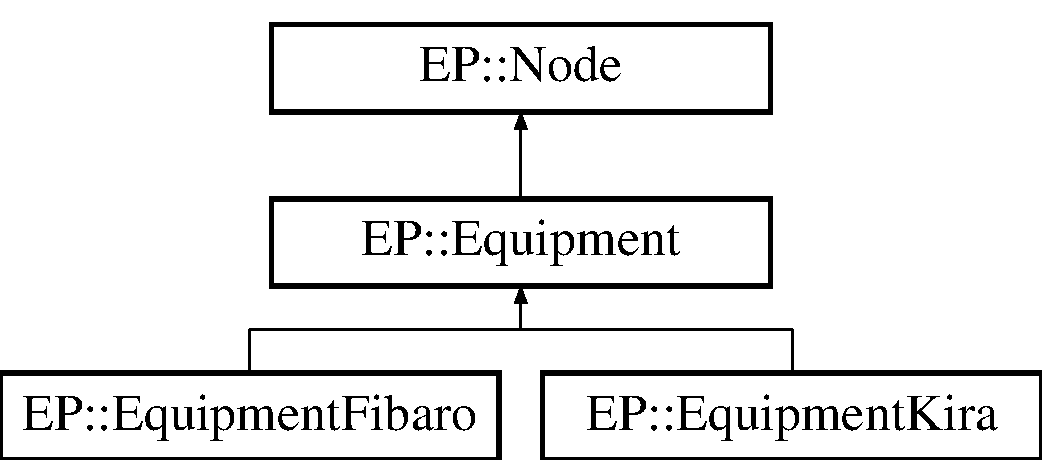
\includegraphics[height=3.000000cm]{class_e_p_1_1_equipment}
\end{center}
\end{figure}
\subsection*{Public Member Functions}
\begin{DoxyCompactItemize}
\item 
\hyperlink{class_e_p_1_1_equipment_a7fce8df2fed82ae05a50f1489307e2ae}{Equipment} (char $\ast$name, char $\ast$ico, \hyperlink{class_e_p_1_1_node}{Node} $\ast$parent, int type\+Of)
\begin{DoxyCompactList}\small\item\em Appelle le constructeur de \hyperlink{class_e_p_1_1_node}{Node}, initialise m\+\_\+room\+Parent et m\+\_\+type\+Of. \end{DoxyCompactList}\item 
virtual int \hyperlink{class_e_p_1_1_equipment_ab95a169fa00d4b7408bf30320f5b7ad8}{send\+Request} ()=0\hypertarget{class_e_p_1_1_equipment_ab95a169fa00d4b7408bf30320f5b7ad8}{}\label{class_e_p_1_1_equipment_ab95a169fa00d4b7408bf30320f5b7ad8}

\begin{DoxyCompactList}\small\item\em Envoie la requête H\+T\+TP permettant d\textquotesingle{}intéragir avec l\textquotesingle{}équipement. \end{DoxyCompactList}\item 
int \hyperlink{class_e_p_1_1_equipment_aac7c97005aec719e51483c9719386015}{get\+Type\+Of} ()
\item 
\hyperlink{class_e_p_1_1_node}{Node} $\ast$ \hyperlink{class_e_p_1_1_equipment_a4a65e982a7ca98587344786d57745b22}{get\+Node\+Parent} ()
\end{DoxyCompactItemize}
\subsection*{Static Public Member Functions}
\begin{DoxyCompactItemize}
\item 
static char $\ast$ \hyperlink{class_e_p_1_1_equipment_adaffca0c6347dae9c4a50e43964470d7}{get\+Ip\+Kira} ()
\item 
static char $\ast$ \hyperlink{class_e_p_1_1_equipment_a7deb5f2f0fd0298440fd57d6e2e6c07d}{get\+Ip\+Fibaro} ()
\item 
static char $\ast$ \hyperlink{class_e_p_1_1_equipment_a81a3c8902b762f36114f265de34a2f4c}{get\+Login\+Fibaro} ()
\item 
static char $\ast$ \hyperlink{class_e_p_1_1_equipment_abc89eb422fe65d3fd3cba0e0024902ff}{get\+Password\+Fibaro} ()
\item 
static int \hyperlink{class_e_p_1_1_equipment_ad7e1a1a1b42188a16233215a908deca0}{set\+Ip\+Kira} (char $\ast$new\+\_\+ip)
\item 
static int \hyperlink{class_e_p_1_1_equipment_ae947b329b91e6d9cb37b618acc34a2a7}{set\+Ip\+Fibaro} (char $\ast$new\+\_\+ip)
\item 
static int \hyperlink{class_e_p_1_1_equipment_ab2bf8dd407ef5b0d998918cd6ab6a8a3}{set\+Login\+Fibaro} (char $\ast$new\+\_\+login)
\item 
static int \hyperlink{class_e_p_1_1_equipment_ad1abd0762bc1f17283307e6a102f0daa}{set\+Password\+Fibaro} (char $\ast$new\+\_\+password)
\end{DoxyCompactItemize}
\subsection*{Protected Attributes}
\begin{DoxyCompactItemize}
\item 
\hyperlink{class_e_p_1_1_node}{Node} $\ast$ \hyperlink{class_e_p_1_1_equipment_a826ee59574194978cd3e02e8824a0a5a}{m\+\_\+room\+Parent}\hypertarget{class_e_p_1_1_equipment_a826ee59574194978cd3e02e8824a0a5a}{}\label{class_e_p_1_1_equipment_a826ee59574194978cd3e02e8824a0a5a}

\begin{DoxyCompactList}\small\item\em Un pointeur vers la pièce contenant l\textquotesingle{}équipement. \end{DoxyCompactList}\item 
int \hyperlink{class_e_p_1_1_equipment_abf8f83a01b6843ffc15cc8b77254dbe3}{m\+\_\+type\+Of}\hypertarget{class_e_p_1_1_equipment_abf8f83a01b6843ffc15cc8b77254dbe3}{}\label{class_e_p_1_1_equipment_abf8f83a01b6843ffc15cc8b77254dbe3}

\begin{DoxyCompactList}\small\item\em 1\+: pour un équipement lié à la Kira, 2\+: pour un équipement lié à la Fibaro. \end{DoxyCompactList}\end{DoxyCompactItemize}
\subsection*{Static Protected Attributes}
\begin{DoxyCompactItemize}
\item 
static char \hyperlink{class_e_p_1_1_equipment_a05245b7dd3a4b4e3fb7ab258e6bbe6a2}{I\+P\+\_\+\+Kira} \mbox{[}15\mbox{]} = \char`\"{}192.\+168.\+1.\+31\char`\"{}\hypertarget{class_e_p_1_1_equipment_a05245b7dd3a4b4e3fb7ab258e6bbe6a2}{}\label{class_e_p_1_1_equipment_a05245b7dd3a4b4e3fb7ab258e6bbe6a2}

\begin{DoxyCompactList}\small\item\em L\textquotesingle{}adresse IP de la Kira. \end{DoxyCompactList}\item 
static char \hyperlink{class_e_p_1_1_equipment_a76405ab4adccec1b32a1c874171749e6}{I\+P\+\_\+\+Fibaro} \mbox{[}15\mbox{]} = \char`\"{}192.\+168.\+81.\+1\char`\"{}\hypertarget{class_e_p_1_1_equipment_a76405ab4adccec1b32a1c874171749e6}{}\label{class_e_p_1_1_equipment_a76405ab4adccec1b32a1c874171749e6}

\begin{DoxyCompactList}\small\item\em L\textquotesingle{}adresse IP de la Fibaro. \end{DoxyCompactList}\item 
static char \hyperlink{class_e_p_1_1_equipment_a91662c50e9eac8a97c2eb5fcc0f1876c}{Fibaro\+\_\+login} \mbox{[}300\mbox{]} = \char`\"{}admin\char`\"{}\hypertarget{class_e_p_1_1_equipment_a91662c50e9eac8a97c2eb5fcc0f1876c}{}\label{class_e_p_1_1_equipment_a91662c50e9eac8a97c2eb5fcc0f1876c}

\begin{DoxyCompactList}\small\item\em Le login de la Fibaro. \end{DoxyCompactList}\item 
static char \hyperlink{class_e_p_1_1_equipment_ad59ffc7e13909e5586601a1e9ce4f9ee}{Fibaro\+\_\+password} \mbox{[}300\mbox{]} = \char`\"{}admin\char`\"{}\hypertarget{class_e_p_1_1_equipment_ad59ffc7e13909e5586601a1e9ce4f9ee}{}\label{class_e_p_1_1_equipment_ad59ffc7e13909e5586601a1e9ce4f9ee}

\begin{DoxyCompactList}\small\item\em Le password de la Fibaro. \end{DoxyCompactList}\end{DoxyCompactItemize}


\subsection{Detailed Description}
Représente un équipement. Cette classe abstraite est spécialisée par \hyperlink{class_e_p_1_1_equipment_kira}{Equipment\+Kira} et \hyperlink{class_e_p_1_1_equipment_fibaro}{Equipment\+Fibaro}. 

\subsection{Constructor \& Destructor Documentation}
\index{E\+P\+::\+Equipment@{E\+P\+::\+Equipment}!Equipment@{Equipment}}
\index{Equipment@{Equipment}!E\+P\+::\+Equipment@{E\+P\+::\+Equipment}}
\subsubsection[{\texorpdfstring{Equipment(char $\ast$name, char $\ast$ico, Node $\ast$parent, int type\+Of)}{Equipment(char *name, char *ico, Node *parent, int typeOf)}}]{\setlength{\rightskip}{0pt plus 5cm}E\+P\+::\+Equipment\+::\+Equipment (
\begin{DoxyParamCaption}
\item[{char $\ast$}]{name, }
\item[{char $\ast$}]{ico, }
\item[{{\bf Node} $\ast$}]{parent, }
\item[{int}]{type\+Of}
\end{DoxyParamCaption}
)\hspace{0.3cm}{\ttfamily [inline]}}\hypertarget{class_e_p_1_1_equipment_a7fce8df2fed82ae05a50f1489307e2ae}{}\label{class_e_p_1_1_equipment_a7fce8df2fed82ae05a50f1489307e2ae}


Appelle le constructeur de \hyperlink{class_e_p_1_1_node}{Node}, initialise m\+\_\+room\+Parent et m\+\_\+type\+Of. 


\begin{DoxyParams}{Parameters}
{\em parent} & La pièce contenant l\textquotesingle{}équipement \\
\hline
{\em type\+Of} & 1\+: pour un équipement lié à la Kira, 2\+: pour un équipement lié à la Fibaro. \\
\hline
\end{DoxyParams}


\subsection{Member Function Documentation}
\index{E\+P\+::\+Equipment@{E\+P\+::\+Equipment}!get\+Ip\+Fibaro@{get\+Ip\+Fibaro}}
\index{get\+Ip\+Fibaro@{get\+Ip\+Fibaro}!E\+P\+::\+Equipment@{E\+P\+::\+Equipment}}
\subsubsection[{\texorpdfstring{get\+Ip\+Fibaro()}{getIpFibaro()}}]{\setlength{\rightskip}{0pt plus 5cm}static char$\ast$ E\+P\+::\+Equipment\+::get\+Ip\+Fibaro (
\begin{DoxyParamCaption}
{}
\end{DoxyParamCaption}
)\hspace{0.3cm}{\ttfamily [inline]}, {\ttfamily [static]}}\hypertarget{class_e_p_1_1_equipment_a7deb5f2f0fd0298440fd57d6e2e6c07d}{}\label{class_e_p_1_1_equipment_a7deb5f2f0fd0298440fd57d6e2e6c07d}
\begin{DoxyReturn}{Returns}
L\textquotesingle{}adresse IP de la Fibaro. 
\end{DoxyReturn}
\index{E\+P\+::\+Equipment@{E\+P\+::\+Equipment}!get\+Ip\+Kira@{get\+Ip\+Kira}}
\index{get\+Ip\+Kira@{get\+Ip\+Kira}!E\+P\+::\+Equipment@{E\+P\+::\+Equipment}}
\subsubsection[{\texorpdfstring{get\+Ip\+Kira()}{getIpKira()}}]{\setlength{\rightskip}{0pt plus 5cm}static char$\ast$ E\+P\+::\+Equipment\+::get\+Ip\+Kira (
\begin{DoxyParamCaption}
{}
\end{DoxyParamCaption}
)\hspace{0.3cm}{\ttfamily [inline]}, {\ttfamily [static]}}\hypertarget{class_e_p_1_1_equipment_adaffca0c6347dae9c4a50e43964470d7}{}\label{class_e_p_1_1_equipment_adaffca0c6347dae9c4a50e43964470d7}
\begin{DoxyReturn}{Returns}
L\textquotesingle{}adresse IP de la Kira. 
\end{DoxyReturn}
\index{E\+P\+::\+Equipment@{E\+P\+::\+Equipment}!get\+Login\+Fibaro@{get\+Login\+Fibaro}}
\index{get\+Login\+Fibaro@{get\+Login\+Fibaro}!E\+P\+::\+Equipment@{E\+P\+::\+Equipment}}
\subsubsection[{\texorpdfstring{get\+Login\+Fibaro()}{getLoginFibaro()}}]{\setlength{\rightskip}{0pt plus 5cm}static char$\ast$ E\+P\+::\+Equipment\+::get\+Login\+Fibaro (
\begin{DoxyParamCaption}
{}
\end{DoxyParamCaption}
)\hspace{0.3cm}{\ttfamily [inline]}, {\ttfamily [static]}}\hypertarget{class_e_p_1_1_equipment_a81a3c8902b762f36114f265de34a2f4c}{}\label{class_e_p_1_1_equipment_a81a3c8902b762f36114f265de34a2f4c}
\begin{DoxyReturn}{Returns}
Le login de la Fibaro. 
\end{DoxyReturn}
\index{E\+P\+::\+Equipment@{E\+P\+::\+Equipment}!get\+Node\+Parent@{get\+Node\+Parent}}
\index{get\+Node\+Parent@{get\+Node\+Parent}!E\+P\+::\+Equipment@{E\+P\+::\+Equipment}}
\subsubsection[{\texorpdfstring{get\+Node\+Parent()}{getNodeParent()}}]{\setlength{\rightskip}{0pt plus 5cm}{\bf Node}$\ast$ E\+P\+::\+Equipment\+::get\+Node\+Parent (
\begin{DoxyParamCaption}
{}
\end{DoxyParamCaption}
)\hspace{0.3cm}{\ttfamily [inline]}}\hypertarget{class_e_p_1_1_equipment_a4a65e982a7ca98587344786d57745b22}{}\label{class_e_p_1_1_equipment_a4a65e982a7ca98587344786d57745b22}
\begin{DoxyReturn}{Returns}
L\textquotesingle{}attribut m\+\_\+room\+Parent. 
\end{DoxyReturn}
\index{E\+P\+::\+Equipment@{E\+P\+::\+Equipment}!get\+Password\+Fibaro@{get\+Password\+Fibaro}}
\index{get\+Password\+Fibaro@{get\+Password\+Fibaro}!E\+P\+::\+Equipment@{E\+P\+::\+Equipment}}
\subsubsection[{\texorpdfstring{get\+Password\+Fibaro()}{getPasswordFibaro()}}]{\setlength{\rightskip}{0pt plus 5cm}static char$\ast$ E\+P\+::\+Equipment\+::get\+Password\+Fibaro (
\begin{DoxyParamCaption}
{}
\end{DoxyParamCaption}
)\hspace{0.3cm}{\ttfamily [inline]}, {\ttfamily [static]}}\hypertarget{class_e_p_1_1_equipment_abc89eb422fe65d3fd3cba0e0024902ff}{}\label{class_e_p_1_1_equipment_abc89eb422fe65d3fd3cba0e0024902ff}
\begin{DoxyReturn}{Returns}
Le password de la Fibaro. 
\end{DoxyReturn}
\index{E\+P\+::\+Equipment@{E\+P\+::\+Equipment}!get\+Type\+Of@{get\+Type\+Of}}
\index{get\+Type\+Of@{get\+Type\+Of}!E\+P\+::\+Equipment@{E\+P\+::\+Equipment}}
\subsubsection[{\texorpdfstring{get\+Type\+Of()}{getTypeOf()}}]{\setlength{\rightskip}{0pt plus 5cm}int E\+P\+::\+Equipment\+::get\+Type\+Of (
\begin{DoxyParamCaption}
{}
\end{DoxyParamCaption}
)\hspace{0.3cm}{\ttfamily [inline]}}\hypertarget{class_e_p_1_1_equipment_aac7c97005aec719e51483c9719386015}{}\label{class_e_p_1_1_equipment_aac7c97005aec719e51483c9719386015}
\begin{DoxyReturn}{Returns}
L\textquotesingle{}attribut m\+\_\+type\+Of. 
\end{DoxyReturn}
\index{E\+P\+::\+Equipment@{E\+P\+::\+Equipment}!set\+Ip\+Fibaro@{set\+Ip\+Fibaro}}
\index{set\+Ip\+Fibaro@{set\+Ip\+Fibaro}!E\+P\+::\+Equipment@{E\+P\+::\+Equipment}}
\subsubsection[{\texorpdfstring{set\+Ip\+Fibaro(char $\ast$new\+\_\+ip)}{setIpFibaro(char *new_ip)}}]{\setlength{\rightskip}{0pt plus 5cm}int E\+P\+::\+Equipment\+::set\+Ip\+Fibaro (
\begin{DoxyParamCaption}
\item[{char $\ast$}]{new\+\_\+ip}
\end{DoxyParamCaption}
)\hspace{0.3cm}{\ttfamily [static]}}\hypertarget{class_e_p_1_1_equipment_ae947b329b91e6d9cb37b618acc34a2a7}{}\label{class_e_p_1_1_equipment_ae947b329b91e6d9cb37b618acc34a2a7}

\begin{DoxyParams}{Parameters}
{\em new\+\_\+ip} & La nouvelle adresse IP de la Fibaro. \\
\hline
\end{DoxyParams}
\begin{DoxyReturn}{Returns}
0 si l\textquotesingle{}adresse est incorrecte, 1 sinon. 
\end{DoxyReturn}
\index{E\+P\+::\+Equipment@{E\+P\+::\+Equipment}!set\+Ip\+Kira@{set\+Ip\+Kira}}
\index{set\+Ip\+Kira@{set\+Ip\+Kira}!E\+P\+::\+Equipment@{E\+P\+::\+Equipment}}
\subsubsection[{\texorpdfstring{set\+Ip\+Kira(char $\ast$new\+\_\+ip)}{setIpKira(char *new_ip)}}]{\setlength{\rightskip}{0pt plus 5cm}int E\+P\+::\+Equipment\+::set\+Ip\+Kira (
\begin{DoxyParamCaption}
\item[{char $\ast$}]{new\+\_\+ip}
\end{DoxyParamCaption}
)\hspace{0.3cm}{\ttfamily [static]}}\hypertarget{class_e_p_1_1_equipment_ad7e1a1a1b42188a16233215a908deca0}{}\label{class_e_p_1_1_equipment_ad7e1a1a1b42188a16233215a908deca0}

\begin{DoxyParams}{Parameters}
{\em new\+\_\+ip} & La nouvelle adresse IP de la Kira. \\
\hline
\end{DoxyParams}
\begin{DoxyReturn}{Returns}
0 si l\textquotesingle{}adresse est incorrecte, 1 sinon. 
\end{DoxyReturn}
\index{E\+P\+::\+Equipment@{E\+P\+::\+Equipment}!set\+Login\+Fibaro@{set\+Login\+Fibaro}}
\index{set\+Login\+Fibaro@{set\+Login\+Fibaro}!E\+P\+::\+Equipment@{E\+P\+::\+Equipment}}
\subsubsection[{\texorpdfstring{set\+Login\+Fibaro(char $\ast$new\+\_\+login)}{setLoginFibaro(char *new_login)}}]{\setlength{\rightskip}{0pt plus 5cm}int E\+P\+::\+Equipment\+::set\+Login\+Fibaro (
\begin{DoxyParamCaption}
\item[{char $\ast$}]{new\+\_\+login}
\end{DoxyParamCaption}
)\hspace{0.3cm}{\ttfamily [static]}}\hypertarget{class_e_p_1_1_equipment_ab2bf8dd407ef5b0d998918cd6ab6a8a3}{}\label{class_e_p_1_1_equipment_ab2bf8dd407ef5b0d998918cd6ab6a8a3}

\begin{DoxyParams}{Parameters}
{\em new\+\_\+login} & Le nouveau login de la Fibaro. \\
\hline
\end{DoxyParams}
\index{E\+P\+::\+Equipment@{E\+P\+::\+Equipment}!set\+Password\+Fibaro@{set\+Password\+Fibaro}}
\index{set\+Password\+Fibaro@{set\+Password\+Fibaro}!E\+P\+::\+Equipment@{E\+P\+::\+Equipment}}
\subsubsection[{\texorpdfstring{set\+Password\+Fibaro(char $\ast$new\+\_\+password)}{setPasswordFibaro(char *new_password)}}]{\setlength{\rightskip}{0pt plus 5cm}int E\+P\+::\+Equipment\+::set\+Password\+Fibaro (
\begin{DoxyParamCaption}
\item[{char $\ast$}]{new\+\_\+password}
\end{DoxyParamCaption}
)\hspace{0.3cm}{\ttfamily [static]}}\hypertarget{class_e_p_1_1_equipment_ad1abd0762bc1f17283307e6a102f0daa}{}\label{class_e_p_1_1_equipment_ad1abd0762bc1f17283307e6a102f0daa}

\begin{DoxyParams}{Parameters}
{\em new\+\_\+password} & Le nouveau password de la Fibaro. \\
\hline
\end{DoxyParams}


The documentation for this class was generated from the following files\+:\begin{DoxyCompactItemize}
\item 
include/Equipment.\+h\item 
src/Equipment.\+cpp\end{DoxyCompactItemize}

\hypertarget{class_e_p_1_1_equipment_fibaro}{}\section{Référence de la classe EP\+:\+:Equipment\+Fibaro}
\label{class_e_p_1_1_equipment_fibaro}\index{E\+P\+::\+Equipment\+Fibaro@{E\+P\+::\+Equipment\+Fibaro}}


Représente un équipement lié à une Fibaro, hérite de \hyperlink{class_e_p_1_1_equipment}{Equipment}.  




{\ttfamily \#include $<$Equipment.\+h$>$}

Graphe d\textquotesingle{}héritage de EP\+:\+:Equipment\+Fibaro\+:\begin{figure}[H]
\begin{center}
\leavevmode
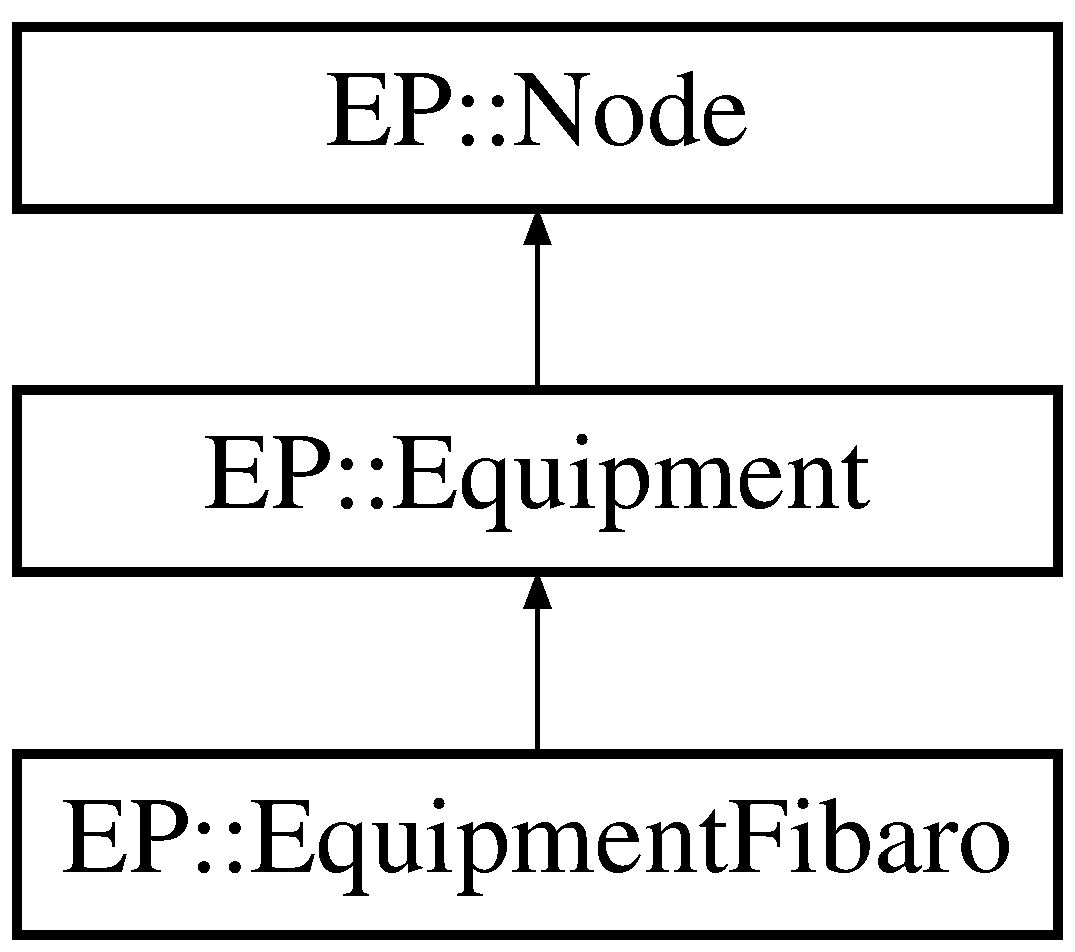
\includegraphics[height=3.000000cm]{class_e_p_1_1_equipment_fibaro}
\end{center}
\end{figure}
\subsection*{Fonctions membres publiques}
\begin{DoxyCompactItemize}
\item 
\hyperlink{class_e_p_1_1_equipment_fibaro_a1aceacf1010faf9042e2a5a4c2f79ae8}{Equipment\+Fibaro} (char $\ast$name, char $\ast$ico, \hyperlink{class_e_p_1_1_node}{Node} $\ast$parent, int equipment\+Id, char $\ast$action)
\begin{DoxyCompactList}\small\item\em Appelle le constructeur de \hyperlink{class_e_p_1_1_equipment}{Equipment} et initialise m\+\_\+equipment\+Id et m\+\_\+action. \end{DoxyCompactList}\item 
virtual int \hyperlink{class_e_p_1_1_equipment_fibaro_aff3a8468127e7915e1757d8b9b600587}{send\+Request} ()\hypertarget{class_e_p_1_1_equipment_fibaro_aff3a8468127e7915e1757d8b9b600587}{}\label{class_e_p_1_1_equipment_fibaro_aff3a8468127e7915e1757d8b9b600587}

\begin{DoxyCompactList}\small\item\em Exécute la requête H\+T\+TP correspondant à cet équipement. \end{DoxyCompactList}\item 
int \hyperlink{class_e_p_1_1_equipment_fibaro_abdd7cbd67d1f3a06dd57fa9dc3b33a59}{get\+Equipment\+Id} ()
\item 
char $\ast$ \hyperlink{class_e_p_1_1_equipment_fibaro_ad411fa6e04286c4b0eabf258226c95f3}{get\+Action} ()
\end{DoxyCompactItemize}
\subsection*{Membres hérités additionnels}


\subsection{Description détaillée}
Représente un équipement lié à une Fibaro, hérite de \hyperlink{class_e_p_1_1_equipment}{Equipment}. 

Définition à la ligne 159 du fichier Equipment.\+h.



\subsection{Documentation des constructeurs et destructeur}
\index{E\+P\+::\+Equipment\+Fibaro@{E\+P\+::\+Equipment\+Fibaro}!Equipment\+Fibaro@{Equipment\+Fibaro}}
\index{Equipment\+Fibaro@{Equipment\+Fibaro}!E\+P\+::\+Equipment\+Fibaro@{E\+P\+::\+Equipment\+Fibaro}}
\subsubsection[{\texorpdfstring{Equipment\+Fibaro(char $\ast$name, char $\ast$ico, Node $\ast$parent, int equipment\+Id, char $\ast$action)}{EquipmentFibaro(char *name, char *ico, Node *parent, int equipmentId, char *action)}}]{\setlength{\rightskip}{0pt plus 5cm}E\+P\+::\+Equipment\+Fibaro\+::\+Equipment\+Fibaro (
\begin{DoxyParamCaption}
\item[{char $\ast$}]{name, }
\item[{char $\ast$}]{ico, }
\item[{{\bf Node} $\ast$}]{parent, }
\item[{int}]{equipment\+Id, }
\item[{char $\ast$}]{action}
\end{DoxyParamCaption}
)}\hypertarget{class_e_p_1_1_equipment_fibaro_a1aceacf1010faf9042e2a5a4c2f79ae8}{}\label{class_e_p_1_1_equipment_fibaro_a1aceacf1010faf9042e2a5a4c2f79ae8}


Appelle le constructeur de \hyperlink{class_e_p_1_1_equipment}{Equipment} et initialise m\+\_\+equipment\+Id et m\+\_\+action. 


\begin{DoxyParams}{Paramètres}
{\em equipment\+Id} & L\textquotesingle{}identifiant correspondant à l\textquotesingle{}équipement dans l\textquotesingle{}interface web de la Fibaro. \\
\hline
{\em action} & L\textquotesingle{}action que l\textquotesingle{}équipement devra effectuer. \\
\hline
\end{DoxyParams}


Définition à la ligne 113 du fichier Equipment.\+cpp.



\subsection{Documentation des fonctions membres}
\index{E\+P\+::\+Equipment\+Fibaro@{E\+P\+::\+Equipment\+Fibaro}!get\+Action@{get\+Action}}
\index{get\+Action@{get\+Action}!E\+P\+::\+Equipment\+Fibaro@{E\+P\+::\+Equipment\+Fibaro}}
\subsubsection[{\texorpdfstring{get\+Action()}{getAction()}}]{\setlength{\rightskip}{0pt plus 5cm}char $\ast$ E\+P\+::\+Equipment\+Fibaro\+::get\+Action (
\begin{DoxyParamCaption}
{}
\end{DoxyParamCaption}
)}\hypertarget{class_e_p_1_1_equipment_fibaro_ad411fa6e04286c4b0eabf258226c95f3}{}\label{class_e_p_1_1_equipment_fibaro_ad411fa6e04286c4b0eabf258226c95f3}
\begin{DoxyReturn}{Renvoie}
L\textquotesingle{}action que l\textquotesingle{}équipement devra effectuer. 
\end{DoxyReturn}


Définition à la ligne 138 du fichier Equipment.\+cpp.

\index{E\+P\+::\+Equipment\+Fibaro@{E\+P\+::\+Equipment\+Fibaro}!get\+Equipment\+Id@{get\+Equipment\+Id}}
\index{get\+Equipment\+Id@{get\+Equipment\+Id}!E\+P\+::\+Equipment\+Fibaro@{E\+P\+::\+Equipment\+Fibaro}}
\subsubsection[{\texorpdfstring{get\+Equipment\+Id()}{getEquipmentId()}}]{\setlength{\rightskip}{0pt plus 5cm}int E\+P\+::\+Equipment\+Fibaro\+::get\+Equipment\+Id (
\begin{DoxyParamCaption}
{}
\end{DoxyParamCaption}
)}\hypertarget{class_e_p_1_1_equipment_fibaro_abdd7cbd67d1f3a06dd57fa9dc3b33a59}{}\label{class_e_p_1_1_equipment_fibaro_abdd7cbd67d1f3a06dd57fa9dc3b33a59}
\begin{DoxyReturn}{Renvoie}
L\textquotesingle{}identifiant correspondant à l\textquotesingle{}équipement dans l\textquotesingle{}interface web de la Fibaro. 
\end{DoxyReturn}


Définition à la ligne 134 du fichier Equipment.\+cpp.



La documentation de cette classe a été générée à partir des fichiers suivants \+:\begin{DoxyCompactItemize}
\item 
include/Equipment.\+h\item 
src/Equipment.\+cpp\end{DoxyCompactItemize}

\hypertarget{class_e_p_1_1_equipment_kira}{}\section{Référence de la classe EP\+:\+:Equipment\+Kira}
\label{class_e_p_1_1_equipment_kira}\index{E\+P\+::\+Equipment\+Kira@{E\+P\+::\+Equipment\+Kira}}


Représente un équipement lié à une Kira, hérite de \hyperlink{class_e_p_1_1_equipment}{Equipment}.  




{\ttfamily \#include $<$Equipment.\+h$>$}

Graphe d\textquotesingle{}héritage de EP\+:\+:Equipment\+Kira\+:\begin{figure}[H]
\begin{center}
\leavevmode
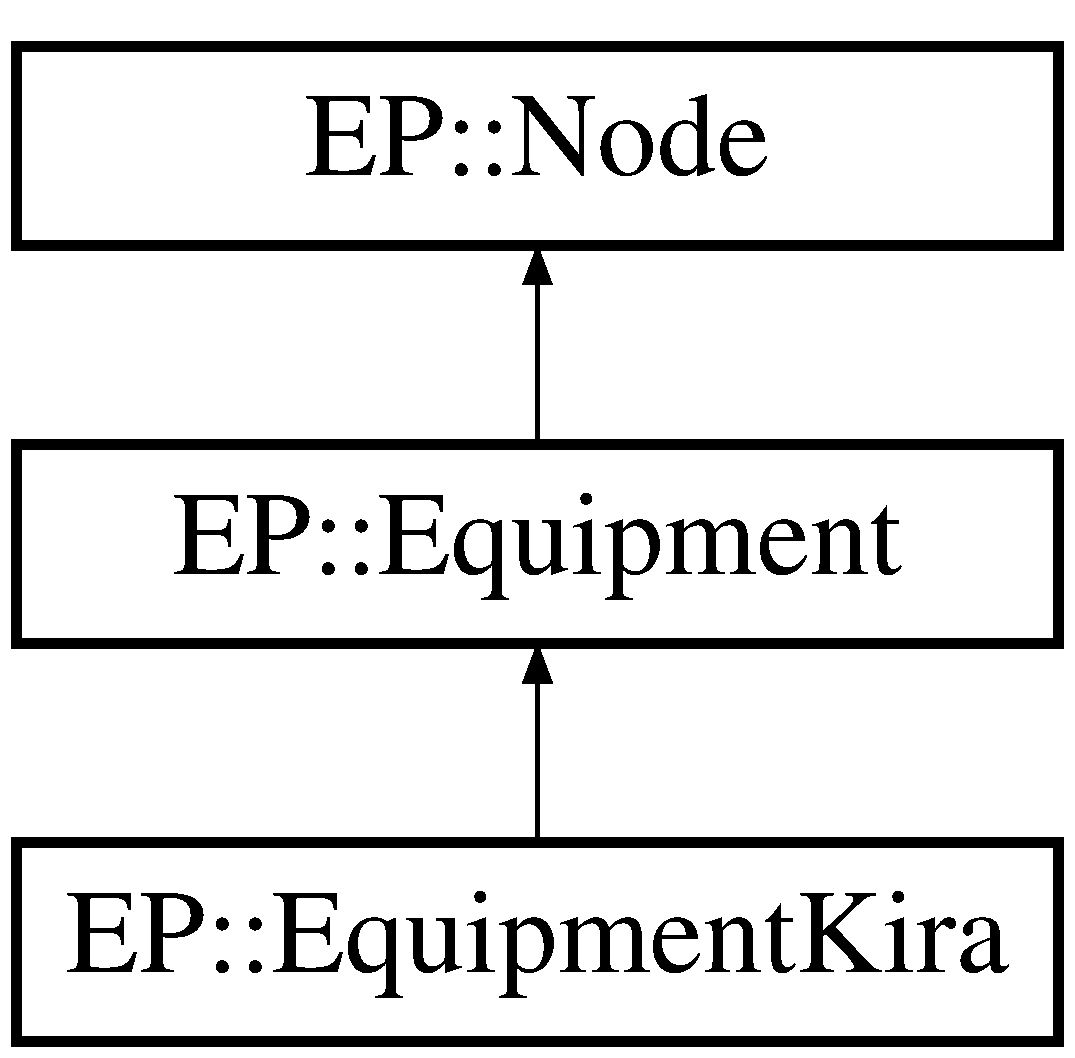
\includegraphics[height=3.000000cm]{class_e_p_1_1_equipment_kira}
\end{center}
\end{figure}
\subsection*{Fonctions membres publiques}
\begin{DoxyCompactItemize}
\item 
\hyperlink{class_e_p_1_1_equipment_kira_a7b96ccdab1a7d69e656c9602fce99213}{Equipment\+Kira} (char $\ast$name, char $\ast$ico, \hyperlink{class_e_p_1_1_node}{Node} $\ast$parent, int button\+Id, int page)
\begin{DoxyCompactList}\small\item\em Appelle le constructeur de \hyperlink{class_e_p_1_1_equipment}{Equipment} et initialise m\+\_\+button\+Id et m\+\_\+page. \end{DoxyCompactList}\item 
virtual int \hyperlink{class_e_p_1_1_equipment_kira_ad59c93de1b98996ec273c5638cd7e47a}{send\+Request} ()\hypertarget{class_e_p_1_1_equipment_kira_ad59c93de1b98996ec273c5638cd7e47a}{}\label{class_e_p_1_1_equipment_kira_ad59c93de1b98996ec273c5638cd7e47a}

\begin{DoxyCompactList}\small\item\em Exécute la requête H\+T\+TP correspondant à cet équipement. \end{DoxyCompactList}\item 
int \hyperlink{class_e_p_1_1_equipment_kira_ae2ce7a10bf38a28b5c0c8f44420c3f10}{get\+Button\+Id} ()
\item 
int \hyperlink{class_e_p_1_1_equipment_kira_a689d07be3886b6b195e9c7bb3c20986d}{get\+Page\+Number} ()
\item 
int \hyperlink{class_e_p_1_1_equipment_kira_a1e695e63e1e736d1d107079a8277db2c}{set\+Button\+Id} (int new\+\_\+id)
\item 
int \hyperlink{class_e_p_1_1_equipment_kira_a788cf486ccf2652a40f4104f27478d74}{set\+Page\+Number} (int new\+\_\+\+Page\+Number)
\end{DoxyCompactItemize}
\subsection*{Membres hérités additionnels}


\subsection{Description détaillée}
Représente un équipement lié à une Kira, hérite de \hyperlink{class_e_p_1_1_equipment}{Equipment}. 

Définition à la ligne 114 du fichier Equipment.\+h.



\subsection{Documentation des constructeurs et destructeur}
\index{E\+P\+::\+Equipment\+Kira@{E\+P\+::\+Equipment\+Kira}!Equipment\+Kira@{Equipment\+Kira}}
\index{Equipment\+Kira@{Equipment\+Kira}!E\+P\+::\+Equipment\+Kira@{E\+P\+::\+Equipment\+Kira}}
\subsubsection[{\texorpdfstring{Equipment\+Kira(char $\ast$name, char $\ast$ico, Node $\ast$parent, int button\+Id, int page)}{EquipmentKira(char *name, char *ico, Node *parent, int buttonId, int page)}}]{\setlength{\rightskip}{0pt plus 5cm}E\+P\+::\+Equipment\+Kira\+::\+Equipment\+Kira (
\begin{DoxyParamCaption}
\item[{char $\ast$}]{name, }
\item[{char $\ast$}]{ico, }
\item[{{\bf Node} $\ast$}]{parent, }
\item[{int}]{button\+Id, }
\item[{int}]{page}
\end{DoxyParamCaption}
)}\hypertarget{class_e_p_1_1_equipment_kira_a7b96ccdab1a7d69e656c9602fce99213}{}\label{class_e_p_1_1_equipment_kira_a7b96ccdab1a7d69e656c9602fce99213}


Appelle le constructeur de \hyperlink{class_e_p_1_1_equipment}{Equipment} et initialise m\+\_\+button\+Id et m\+\_\+page. 


\begin{DoxyParams}{Paramètres}
{\em button\+Id} & Le numéro du bouton correspondant à l\textquotesingle{}équipement dans l\textquotesingle{}interface web de la Kira. \\
\hline
{\em page} & La page du bouton correspondant à l\textquotesingle{}équipement dans l\textquotesingle{}interface web de la Kira. \\
\hline
\end{DoxyParams}


Définition à la ligne 64 du fichier Equipment.\+cpp.



\subsection{Documentation des fonctions membres}
\index{E\+P\+::\+Equipment\+Kira@{E\+P\+::\+Equipment\+Kira}!get\+Button\+Id@{get\+Button\+Id}}
\index{get\+Button\+Id@{get\+Button\+Id}!E\+P\+::\+Equipment\+Kira@{E\+P\+::\+Equipment\+Kira}}
\subsubsection[{\texorpdfstring{get\+Button\+Id()}{getButtonId()}}]{\setlength{\rightskip}{0pt plus 5cm}int E\+P\+::\+Equipment\+Kira\+::get\+Button\+Id (
\begin{DoxyParamCaption}
{}
\end{DoxyParamCaption}
)}\hypertarget{class_e_p_1_1_equipment_kira_ae2ce7a10bf38a28b5c0c8f44420c3f10}{}\label{class_e_p_1_1_equipment_kira_ae2ce7a10bf38a28b5c0c8f44420c3f10}
\begin{DoxyReturn}{Renvoie}
Le numéro du bouton correspondant à l\textquotesingle{}équipement dans l\textquotesingle{}interface web de la Kira. 
\end{DoxyReturn}


Définition à la ligne 86 du fichier Equipment.\+cpp.

\index{E\+P\+::\+Equipment\+Kira@{E\+P\+::\+Equipment\+Kira}!get\+Page\+Number@{get\+Page\+Number}}
\index{get\+Page\+Number@{get\+Page\+Number}!E\+P\+::\+Equipment\+Kira@{E\+P\+::\+Equipment\+Kira}}
\subsubsection[{\texorpdfstring{get\+Page\+Number()}{getPageNumber()}}]{\setlength{\rightskip}{0pt plus 5cm}int E\+P\+::\+Equipment\+Kira\+::get\+Page\+Number (
\begin{DoxyParamCaption}
{}
\end{DoxyParamCaption}
)}\hypertarget{class_e_p_1_1_equipment_kira_a689d07be3886b6b195e9c7bb3c20986d}{}\label{class_e_p_1_1_equipment_kira_a689d07be3886b6b195e9c7bb3c20986d}
\begin{DoxyReturn}{Renvoie}
Le numéro de page du bouton correspondant à l\textquotesingle{}équipement dans l\textquotesingle{}interface web de la Kira. 
\end{DoxyReturn}


Définition à la ligne 90 du fichier Equipment.\+cpp.

\index{E\+P\+::\+Equipment\+Kira@{E\+P\+::\+Equipment\+Kira}!set\+Button\+Id@{set\+Button\+Id}}
\index{set\+Button\+Id@{set\+Button\+Id}!E\+P\+::\+Equipment\+Kira@{E\+P\+::\+Equipment\+Kira}}
\subsubsection[{\texorpdfstring{set\+Button\+Id(int new\+\_\+id)}{setButtonId(int new_id)}}]{\setlength{\rightskip}{0pt plus 5cm}int E\+P\+::\+Equipment\+Kira\+::set\+Button\+Id (
\begin{DoxyParamCaption}
\item[{int}]{new\+\_\+id}
\end{DoxyParamCaption}
)}\hypertarget{class_e_p_1_1_equipment_kira_a1e695e63e1e736d1d107079a8277db2c}{}\label{class_e_p_1_1_equipment_kira_a1e695e63e1e736d1d107079a8277db2c}

\begin{DoxyParams}{Paramètres}
{\em new\+\_\+id} & Le nouveau numéro du bouton. \\
\hline
\end{DoxyParams}


Définition à la ligne 94 du fichier Equipment.\+cpp.

\index{E\+P\+::\+Equipment\+Kira@{E\+P\+::\+Equipment\+Kira}!set\+Page\+Number@{set\+Page\+Number}}
\index{set\+Page\+Number@{set\+Page\+Number}!E\+P\+::\+Equipment\+Kira@{E\+P\+::\+Equipment\+Kira}}
\subsubsection[{\texorpdfstring{set\+Page\+Number(int new\+\_\+\+Page\+Number)}{setPageNumber(int new_PageNumber)}}]{\setlength{\rightskip}{0pt plus 5cm}int E\+P\+::\+Equipment\+Kira\+::set\+Page\+Number (
\begin{DoxyParamCaption}
\item[{int}]{new\+\_\+\+Page\+Number}
\end{DoxyParamCaption}
)}\hypertarget{class_e_p_1_1_equipment_kira_a788cf486ccf2652a40f4104f27478d74}{}\label{class_e_p_1_1_equipment_kira_a788cf486ccf2652a40f4104f27478d74}

\begin{DoxyParams}{Paramètres}
{\em new\+\_\+\+Page\+Number} & Le nouveau numéro de page du bouton. \\
\hline
\end{DoxyParams}


Définition à la ligne 99 du fichier Equipment.\+cpp.



La documentation de cette classe a été générée à partir des fichiers suivants \+:\begin{DoxyCompactItemize}
\item 
include/Equipment.\+h\item 
src/Equipment.\+cpp\end{DoxyCompactItemize}

\hypertarget{class_e_p_1_1_node}{}\section{Référence de la classe EP\+:\+:Node}
\label{class_e_p_1_1_node}\index{E\+P\+::\+Node@{E\+P\+::\+Node}}


Représente un noeud de l\textquotesingle{}arbre (une pièce ou un équipement). Cette classe est spécialisée par les classes \hyperlink{class_e_p_1_1_equipment}{Equipment} et \hyperlink{class_e_p_1_1_room}{Room}, et n\textquotesingle{}est donc pas utilisée telle qu\textquotesingle{}elle.  




{\ttfamily \#include $<$Node.\+h$>$}

Graphe d\textquotesingle{}héritage de EP\+:\+:Node\+:\begin{figure}[H]
\begin{center}
\leavevmode
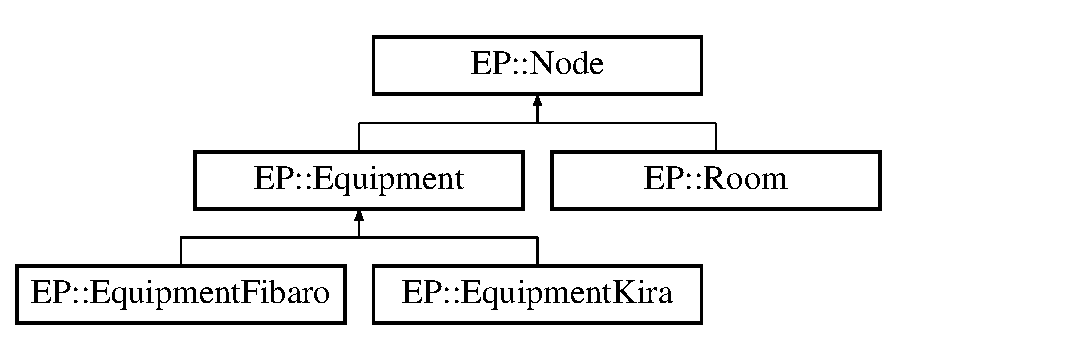
\includegraphics[height=3.000000cm]{class_e_p_1_1_node}
\end{center}
\end{figure}
\subsection*{Fonctions membres publiques}
\begin{DoxyCompactItemize}
\item 
\hyperlink{class_e_p_1_1_node_a9df197a78c36646fba1670935f5ea948}{Node} (char $\ast$name, char $\ast$ico)\hypertarget{class_e_p_1_1_node_a9df197a78c36646fba1670935f5ea948}{}\label{class_e_p_1_1_node_a9df197a78c36646fba1670935f5ea948}

\begin{DoxyCompactList}\small\item\em Constructeur, initialise les attributs m\+\_\+name et m\+\_\+ico. \end{DoxyCompactList}\item 
virtual \hyperlink{class_e_p_1_1_node_a247e246a75f5b7111d53a1e4de19fb0b}{$\sim$\+Node} (void)\hypertarget{class_e_p_1_1_node_a247e246a75f5b7111d53a1e4de19fb0b}{}\label{class_e_p_1_1_node_a247e246a75f5b7111d53a1e4de19fb0b}

\begin{DoxyCompactList}\small\item\em Destructeur, ne fait rien de particulier. \end{DoxyCompactList}\item 
char $\ast$ \hyperlink{class_e_p_1_1_node_ad5dd5dfbe1e26a22de54035a16ddb980}{get\+Name} ()
\item 
void \hyperlink{class_e_p_1_1_node_a27a879726020308b8fd47812ec4a8b86}{set\+Name} (char $\ast$name)
\begin{DoxyCompactList}\small\item\em Change le nom de ce noeud pour celui passé en paramètre. \end{DoxyCompactList}\item 
char $\ast$ \hyperlink{class_e_p_1_1_node_a7e29d725cfe687589f5668c9825fc303}{get\+Ico} ()
\item 
void \hyperlink{class_e_p_1_1_node_a0f1a35a7f9e6d18d38a17b591a130862}{set\+Ico} (char $\ast$ico)
\begin{DoxyCompactList}\small\item\em Change l\textquotesingle{}icône du noeud. \end{DoxyCompactList}\end{DoxyCompactItemize}
\subsection*{Attributs protégés}
\begin{DoxyCompactItemize}
\item 
char \hyperlink{class_e_p_1_1_node_a31312ed65b64cb081b4cbdf0acffa44f}{m\+\_\+name} \mbox{[}100\mbox{]}\hypertarget{class_e_p_1_1_node_a31312ed65b64cb081b4cbdf0acffa44f}{}\label{class_e_p_1_1_node_a31312ed65b64cb081b4cbdf0acffa44f}

\begin{DoxyCompactList}\small\item\em Le nom du noeud. \end{DoxyCompactList}\item 
char \hyperlink{class_e_p_1_1_node_a149cce768568286687e756c1f9dce2b4}{m\+\_\+ico} \mbox{[}100\mbox{]}\hypertarget{class_e_p_1_1_node_a149cce768568286687e756c1f9dce2b4}{}\label{class_e_p_1_1_node_a149cce768568286687e756c1f9dce2b4}

\begin{DoxyCompactList}\small\item\em L\textquotesingle{}icône du noeud qui sera affichée dans l\textquotesingle{}application. \end{DoxyCompactList}\item 
\hyperlink{class_e_p_1_1_node}{E\+P\+::\+Node} $\ast$ \hyperlink{class_e_p_1_1_node_ac61ce03b473134cb3cd4fcf33acc03f6}{m\+\_\+parent}\hypertarget{class_e_p_1_1_node_ac61ce03b473134cb3cd4fcf33acc03f6}{}\label{class_e_p_1_1_node_ac61ce03b473134cb3cd4fcf33acc03f6}

\begin{DoxyCompactList}\small\item\em Le noeud parent de celui-\/ci. Sera nul pour les pièces (\hyperlink{class_e_p_1_1_room}{Room}), et correspondra à la pièce contenante dans le cas d\textquotesingle{}un équipement (\hyperlink{class_e_p_1_1_equipment}{Equipment}). \end{DoxyCompactList}\end{DoxyCompactItemize}


\subsection{Description détaillée}
Représente un noeud de l\textquotesingle{}arbre (une pièce ou un équipement). Cette classe est spécialisée par les classes \hyperlink{class_e_p_1_1_equipment}{Equipment} et \hyperlink{class_e_p_1_1_room}{Room}, et n\textquotesingle{}est donc pas utilisée telle qu\textquotesingle{}elle. 

Définition à la ligne 14 du fichier Node.\+h.



\subsection{Documentation des fonctions membres}
\index{E\+P\+::\+Node@{E\+P\+::\+Node}!get\+Ico@{get\+Ico}}
\index{get\+Ico@{get\+Ico}!E\+P\+::\+Node@{E\+P\+::\+Node}}
\subsubsection[{\texorpdfstring{get\+Ico()}{getIco()}}]{\setlength{\rightskip}{0pt plus 5cm}char $\ast$ E\+P\+::\+Node\+::get\+Ico (
\begin{DoxyParamCaption}
{}
\end{DoxyParamCaption}
)}\hypertarget{class_e_p_1_1_node_a7e29d725cfe687589f5668c9825fc303}{}\label{class_e_p_1_1_node_a7e29d725cfe687589f5668c9825fc303}
\begin{DoxyReturn}{Renvoie}
Le nom du fichier correspondant à l\textquotesingle{}icône de ce noeud. 
\end{DoxyReturn}


Définition à la ligne 18 du fichier Node.\+cpp.

\index{E\+P\+::\+Node@{E\+P\+::\+Node}!get\+Name@{get\+Name}}
\index{get\+Name@{get\+Name}!E\+P\+::\+Node@{E\+P\+::\+Node}}
\subsubsection[{\texorpdfstring{get\+Name()}{getName()}}]{\setlength{\rightskip}{0pt plus 5cm}char $\ast$ E\+P\+::\+Node\+::get\+Name (
\begin{DoxyParamCaption}
{}
\end{DoxyParamCaption}
)}\hypertarget{class_e_p_1_1_node_ad5dd5dfbe1e26a22de54035a16ddb980}{}\label{class_e_p_1_1_node_ad5dd5dfbe1e26a22de54035a16ddb980}
\begin{DoxyReturn}{Renvoie}
Le nom du noeud. 
\end{DoxyReturn}


Définition à la ligne 14 du fichier Node.\+cpp.

\index{E\+P\+::\+Node@{E\+P\+::\+Node}!set\+Ico@{set\+Ico}}
\index{set\+Ico@{set\+Ico}!E\+P\+::\+Node@{E\+P\+::\+Node}}
\subsubsection[{\texorpdfstring{set\+Ico(char $\ast$ico)}{setIco(char *ico)}}]{\setlength{\rightskip}{0pt plus 5cm}void E\+P\+::\+Node\+::set\+Ico (
\begin{DoxyParamCaption}
\item[{char $\ast$}]{ico}
\end{DoxyParamCaption}
)}\hypertarget{class_e_p_1_1_node_a0f1a35a7f9e6d18d38a17b591a130862}{}\label{class_e_p_1_1_node_a0f1a35a7f9e6d18d38a17b591a130862}


Change l\textquotesingle{}icône du noeud. 


\begin{DoxyParams}{Paramètres}
{\em ico} & La nouvelle icône du noeud. \\
\hline
\end{DoxyParams}


Définition à la ligne 26 du fichier Node.\+cpp.

\index{E\+P\+::\+Node@{E\+P\+::\+Node}!set\+Name@{set\+Name}}
\index{set\+Name@{set\+Name}!E\+P\+::\+Node@{E\+P\+::\+Node}}
\subsubsection[{\texorpdfstring{set\+Name(char $\ast$name)}{setName(char *name)}}]{\setlength{\rightskip}{0pt plus 5cm}void E\+P\+::\+Node\+::set\+Name (
\begin{DoxyParamCaption}
\item[{char $\ast$}]{name}
\end{DoxyParamCaption}
)}\hypertarget{class_e_p_1_1_node_a27a879726020308b8fd47812ec4a8b86}{}\label{class_e_p_1_1_node_a27a879726020308b8fd47812ec4a8b86}


Change le nom de ce noeud pour celui passé en paramètre. 


\begin{DoxyParams}{Paramètres}
{\em name} & Le nouveau nom du noeud. \\
\hline
\end{DoxyParams}


Définition à la ligne 22 du fichier Node.\+cpp.



La documentation de cette classe a été générée à partir des fichiers suivants \+:\begin{DoxyCompactItemize}
\item 
include/Node.\+h\item 
src/Node.\+cpp\end{DoxyCompactItemize}

\hypertarget{class_e_p_1_1_room}{}\section{EP\+:\+:Room Class Reference}
\label{class_e_p_1_1_room}\index{E\+P\+::\+Room@{E\+P\+::\+Room}}


Représente une pièce de la maison ; Hérite de \hyperlink{class_e_p_1_1_node}{Node}. On peut y retrouver les différents équipements liés à une pièce et les gérer.  




{\ttfamily \#include $<$Room.\+h$>$}

Inheritance diagram for EP\+:\+:Room\+:\begin{figure}[H]
\begin{center}
\leavevmode
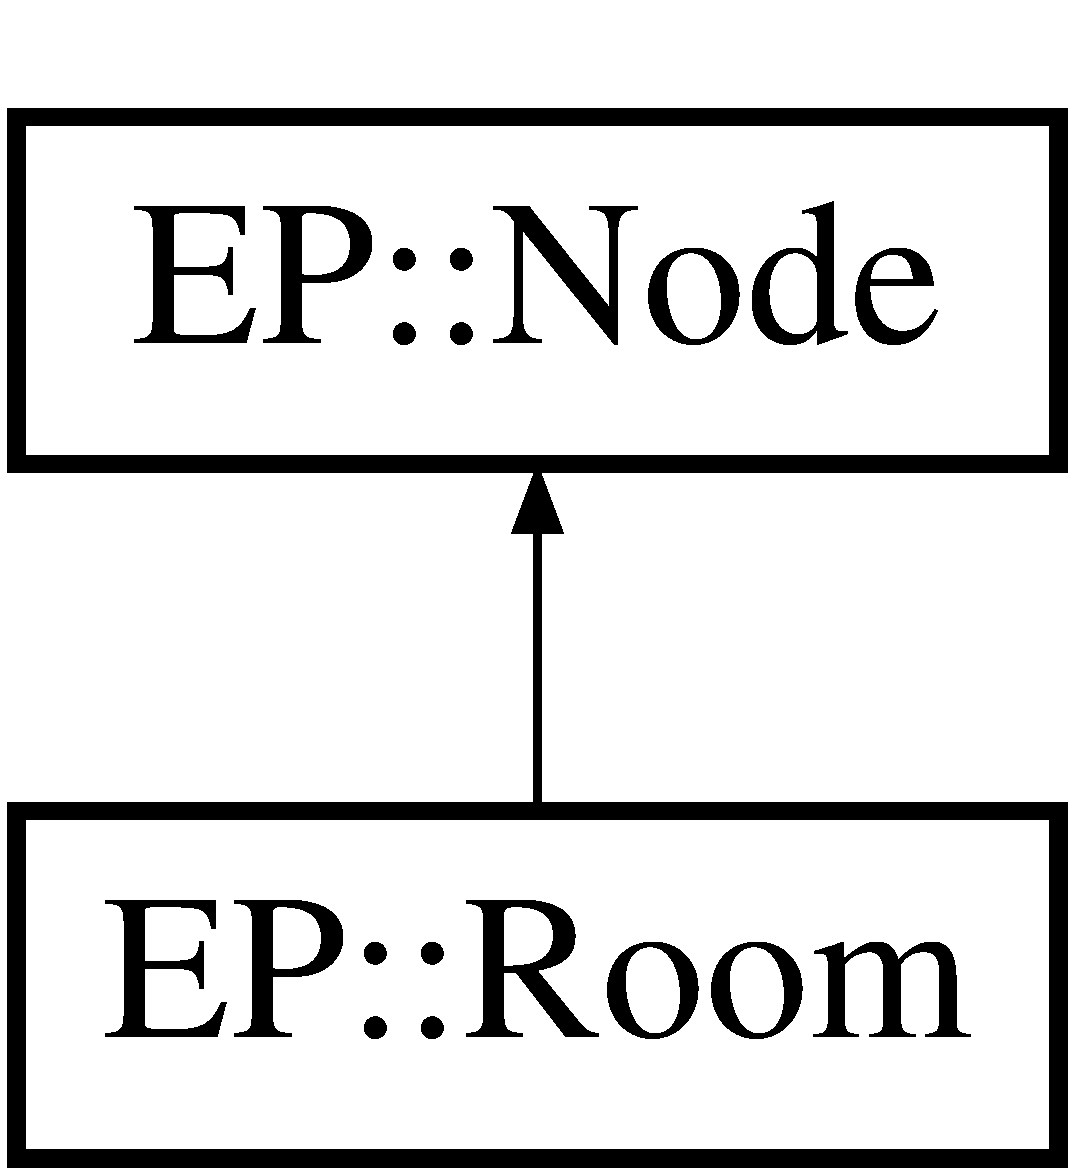
\includegraphics[height=2.000000cm]{class_e_p_1_1_room}
\end{center}
\end{figure}
\subsection*{Public Member Functions}
\begin{DoxyCompactItemize}
\item 
\hyperlink{class_e_p_1_1_room_aefc0919f87a1f6dcfde24923719e6b90}{Room} (char $\ast$name, char $\ast$\hyperlink{namespace_e_p_a9bb18717237cbb94269e26c77cc04b05}{ico})
\begin{DoxyCompactList}\small\item\em Appele le constructeur de \hyperlink{class_e_p_1_1_node}{Node}. \end{DoxyCompactList}\item 
\hyperlink{class_e_p_1_1_room_a1dba2dc4fdec31c930b5f538bb4018cf}{$\sim$\+Room} ()
\begin{DoxyCompactList}\small\item\em Détruit la liste d\textquotesingle{}équipements. \end{DoxyCompactList}\item 
int \hyperlink{class_e_p_1_1_room_a818eb638f5796bfc45a519ce503c30be}{add\+Equipment} (\hyperlink{class_e_p_1_1_equipment}{Equipment} $\ast$equip)
\begin{DoxyCompactList}\small\item\em Ajoute le pointeur d\textquotesingle{}un équipement donné dans m\+\_\+list\+Equipments. Le nom d\textquotesingle{}un équipement doit être unique. \end{DoxyCompactList}\item 
int \hyperlink{class_e_p_1_1_room_a9d9a93b373460edb886a05e8942aa589}{delete\+Equipment\+By\+Index} (int index)
\begin{DoxyCompactList}\small\item\em Supprime l\textquotesingle{}équipement dont l\textquotesingle{}index est donné en paramètre. \end{DoxyCompactList}\item 
int \hyperlink{class_e_p_1_1_room_a4879b1eeebccc1a3c2f5ece234f73da9}{delete\+Equipment\+By\+Name} (char $\ast$name)
\begin{DoxyCompactList}\small\item\em Supprime l\textquotesingle{}équipement dont le nom est donné en paramètre. \end{DoxyCompactList}\item 
std\+::vector$<$ \hyperlink{class_e_p_1_1_equipment}{Equipment} $\ast$ $>$ $\ast$ \hyperlink{class_e_p_1_1_room_ad4993f6208f136a9f1bd082def0d53c0}{get\+Equipments} ()
\begin{DoxyCompactList}\small\item\em Ne pas utiliser cette méthode à partir de la D\+LL. A la place on peut itérer avec get\+Number\+Equipments et get\+Equipment\+By\+Index. \end{DoxyCompactList}\item 
\hyperlink{class_e_p_1_1_equipment}{Equipment} $\ast$ \hyperlink{class_e_p_1_1_room_a7f7aeb553f256013f1f54c245e238dfd}{get\+Equipment\+By\+Name} (char $\ast$name)
\begin{DoxyCompactList}\small\item\em Donne un pointeur vers l\textquotesingle{}équipement dont le nom est donné en paramètre. \end{DoxyCompactList}\item 
\hyperlink{class_e_p_1_1_equipment}{Equipment} $\ast$ \hyperlink{class_e_p_1_1_room_a22185f0f9e75c03fe2fd61c958df3ead}{get\+Equipment\+By\+Index} (int index)
\begin{DoxyCompactList}\small\item\em Donne un pointeur vers l\textquotesingle{}équipement dont l\textquotesingle{}index est donné en paramètre. \end{DoxyCompactList}\item 
int \hyperlink{class_e_p_1_1_room_af66a08a85258e5da63a3684a9efc98ef}{get\+Number\+Equipments} ()
\end{DoxyCompactItemize}
\subsection*{Additional Inherited Members}


\subsection{Detailed Description}
Représente une pièce de la maison ; Hérite de \hyperlink{class_e_p_1_1_node}{Node}. On peut y retrouver les différents équipements liés à une pièce et les gérer. 

\subsection{Constructor \& Destructor Documentation}
\index{E\+P\+::\+Room@{E\+P\+::\+Room}!Room@{Room}}
\index{Room@{Room}!E\+P\+::\+Room@{E\+P\+::\+Room}}
\subsubsection[{\texorpdfstring{Room(char $\ast$name, char $\ast$ico)}{Room(char *name, char *ico)}}]{\setlength{\rightskip}{0pt plus 5cm}E\+P\+::\+Room\+::\+Room (
\begin{DoxyParamCaption}
\item[{char $\ast$}]{name, }
\item[{char $\ast$}]{ico}
\end{DoxyParamCaption}
)}\hypertarget{class_e_p_1_1_room_aefc0919f87a1f6dcfde24923719e6b90}{}\label{class_e_p_1_1_room_aefc0919f87a1f6dcfde24923719e6b90}


Appele le constructeur de \hyperlink{class_e_p_1_1_node}{Node}. 

\index{E\+P\+::\+Room@{E\+P\+::\+Room}!````~Room@{$\sim$\+Room}}
\index{````~Room@{$\sim$\+Room}!E\+P\+::\+Room@{E\+P\+::\+Room}}
\subsubsection[{\texorpdfstring{$\sim$\+Room()}{~Room()}}]{\setlength{\rightskip}{0pt plus 5cm}E\+P\+::\+Room\+::$\sim$\+Room (
\begin{DoxyParamCaption}
{}
\end{DoxyParamCaption}
)}\hypertarget{class_e_p_1_1_room_a1dba2dc4fdec31c930b5f538bb4018cf}{}\label{class_e_p_1_1_room_a1dba2dc4fdec31c930b5f538bb4018cf}


Détruit la liste d\textquotesingle{}équipements. 



\subsection{Member Function Documentation}
\index{E\+P\+::\+Room@{E\+P\+::\+Room}!add\+Equipment@{add\+Equipment}}
\index{add\+Equipment@{add\+Equipment}!E\+P\+::\+Room@{E\+P\+::\+Room}}
\subsubsection[{\texorpdfstring{add\+Equipment(\+Equipment $\ast$equip)}{addEquipment(Equipment *equip)}}]{\setlength{\rightskip}{0pt plus 5cm}int E\+P\+::\+Room\+::add\+Equipment (
\begin{DoxyParamCaption}
\item[{{\bf Equipment} $\ast$}]{equip}
\end{DoxyParamCaption}
)}\hypertarget{class_e_p_1_1_room_a818eb638f5796bfc45a519ce503c30be}{}\label{class_e_p_1_1_room_a818eb638f5796bfc45a519ce503c30be}


Ajoute le pointeur d\textquotesingle{}un équipement donné dans m\+\_\+list\+Equipments. Le nom d\textquotesingle{}un équipement doit être unique. 


\begin{DoxyParams}{Parameters}
{\em equip} & Le pointeur de l\textquotesingle{}équipement à ajouter. \\
\hline
\end{DoxyParams}
\begin{DoxyReturn}{Returns}
0 si tout s\textquotesingle{}est bien passé, 1 si le nom est déjà pris. 
\end{DoxyReturn}
\index{E\+P\+::\+Room@{E\+P\+::\+Room}!delete\+Equipment\+By\+Index@{delete\+Equipment\+By\+Index}}
\index{delete\+Equipment\+By\+Index@{delete\+Equipment\+By\+Index}!E\+P\+::\+Room@{E\+P\+::\+Room}}
\subsubsection[{\texorpdfstring{delete\+Equipment\+By\+Index(int index)}{deleteEquipmentByIndex(int index)}}]{\setlength{\rightskip}{0pt plus 5cm}int E\+P\+::\+Room\+::delete\+Equipment\+By\+Index (
\begin{DoxyParamCaption}
\item[{int}]{index}
\end{DoxyParamCaption}
)}\hypertarget{class_e_p_1_1_room_a9d9a93b373460edb886a05e8942aa589}{}\label{class_e_p_1_1_room_a9d9a93b373460edb886a05e8942aa589}


Supprime l\textquotesingle{}équipement dont l\textquotesingle{}index est donné en paramètre. 


\begin{DoxyParams}{Parameters}
{\em index} & L\textquotesingle{}index de l\textquotesingle{}équipement à supprimer de m\+\_\+list\+Equipments. \\
\hline
\end{DoxyParams}
\begin{DoxyReturn}{Returns}
0 si tout s\textquotesingle{}est bien passé, 1 si l\textquotesingle{}index ne correspond à aucun équipement. 
\end{DoxyReturn}
\index{E\+P\+::\+Room@{E\+P\+::\+Room}!delete\+Equipment\+By\+Name@{delete\+Equipment\+By\+Name}}
\index{delete\+Equipment\+By\+Name@{delete\+Equipment\+By\+Name}!E\+P\+::\+Room@{E\+P\+::\+Room}}
\subsubsection[{\texorpdfstring{delete\+Equipment\+By\+Name(char $\ast$name)}{deleteEquipmentByName(char *name)}}]{\setlength{\rightskip}{0pt plus 5cm}int E\+P\+::\+Room\+::delete\+Equipment\+By\+Name (
\begin{DoxyParamCaption}
\item[{char $\ast$}]{name}
\end{DoxyParamCaption}
)}\hypertarget{class_e_p_1_1_room_a4879b1eeebccc1a3c2f5ece234f73da9}{}\label{class_e_p_1_1_room_a4879b1eeebccc1a3c2f5ece234f73da9}


Supprime l\textquotesingle{}équipement dont le nom est donné en paramètre. 


\begin{DoxyParams}{Parameters}
{\em name} & Le nom de l\textquotesingle{}équipement à supprimer de m\+\_\+list\+Equipments. \\
\hline
\end{DoxyParams}
\begin{DoxyReturn}{Returns}
0 si tout s\textquotesingle{}est bien passé, 1 si le nom ne correspond à aucun équipement. 
\end{DoxyReturn}
\index{E\+P\+::\+Room@{E\+P\+::\+Room}!get\+Equipment\+By\+Index@{get\+Equipment\+By\+Index}}
\index{get\+Equipment\+By\+Index@{get\+Equipment\+By\+Index}!E\+P\+::\+Room@{E\+P\+::\+Room}}
\subsubsection[{\texorpdfstring{get\+Equipment\+By\+Index(int index)}{getEquipmentByIndex(int index)}}]{\setlength{\rightskip}{0pt plus 5cm}{\bf Equipment} $\ast$ E\+P\+::\+Room\+::get\+Equipment\+By\+Index (
\begin{DoxyParamCaption}
\item[{int}]{index}
\end{DoxyParamCaption}
)}\hypertarget{class_e_p_1_1_room_a22185f0f9e75c03fe2fd61c958df3ead}{}\label{class_e_p_1_1_room_a22185f0f9e75c03fe2fd61c958df3ead}


Donne un pointeur vers l\textquotesingle{}équipement dont l\textquotesingle{}index est donné en paramètre. 


\begin{DoxyParams}{Parameters}
{\em index} & L\textquotesingle{}index de l\textquotesingle{}équipement qu\textquotesingle{}on veut récupérer. \\
\hline
\end{DoxyParams}
\begin{DoxyReturn}{Returns}
Un pointeur vers l\textquotesingle{}équipement demandé, N\+U\+LL si aucun ne correspond. 
\end{DoxyReturn}
\index{E\+P\+::\+Room@{E\+P\+::\+Room}!get\+Equipment\+By\+Name@{get\+Equipment\+By\+Name}}
\index{get\+Equipment\+By\+Name@{get\+Equipment\+By\+Name}!E\+P\+::\+Room@{E\+P\+::\+Room}}
\subsubsection[{\texorpdfstring{get\+Equipment\+By\+Name(char $\ast$name)}{getEquipmentByName(char *name)}}]{\setlength{\rightskip}{0pt plus 5cm}{\bf Equipment} $\ast$ E\+P\+::\+Room\+::get\+Equipment\+By\+Name (
\begin{DoxyParamCaption}
\item[{char $\ast$}]{name}
\end{DoxyParamCaption}
)}\hypertarget{class_e_p_1_1_room_a7f7aeb553f256013f1f54c245e238dfd}{}\label{class_e_p_1_1_room_a7f7aeb553f256013f1f54c245e238dfd}


Donne un pointeur vers l\textquotesingle{}équipement dont le nom est donné en paramètre. 


\begin{DoxyParams}{Parameters}
{\em name} & Le nom de l\textquotesingle{}équipement qu\textquotesingle{}on veut récupérer. \\
\hline
\end{DoxyParams}
\begin{DoxyReturn}{Returns}
Un pointeur vers l\textquotesingle{}équipement demandé, N\+U\+LL si aucun ne correspond. 
\end{DoxyReturn}
\index{E\+P\+::\+Room@{E\+P\+::\+Room}!get\+Equipments@{get\+Equipments}}
\index{get\+Equipments@{get\+Equipments}!E\+P\+::\+Room@{E\+P\+::\+Room}}
\subsubsection[{\texorpdfstring{get\+Equipments()}{getEquipments()}}]{\setlength{\rightskip}{0pt plus 5cm}vector$<$ {\bf Equipment} $\ast$ $>$ $\ast$ E\+P\+::\+Room\+::get\+Equipments (
\begin{DoxyParamCaption}
{}
\end{DoxyParamCaption}
)}\hypertarget{class_e_p_1_1_room_ad4993f6208f136a9f1bd082def0d53c0}{}\label{class_e_p_1_1_room_ad4993f6208f136a9f1bd082def0d53c0}


Ne pas utiliser cette méthode à partir de la D\+LL. A la place on peut itérer avec get\+Number\+Equipments et get\+Equipment\+By\+Index. 

\begin{DoxyReturn}{Returns}
L\textquotesingle{}attribut m\+\_\+list\+Equipments. 
\end{DoxyReturn}
\index{E\+P\+::\+Room@{E\+P\+::\+Room}!get\+Number\+Equipments@{get\+Number\+Equipments}}
\index{get\+Number\+Equipments@{get\+Number\+Equipments}!E\+P\+::\+Room@{E\+P\+::\+Room}}
\subsubsection[{\texorpdfstring{get\+Number\+Equipments()}{getNumberEquipments()}}]{\setlength{\rightskip}{0pt plus 5cm}int E\+P\+::\+Room\+::get\+Number\+Equipments (
\begin{DoxyParamCaption}
{}
\end{DoxyParamCaption}
)}\hypertarget{class_e_p_1_1_room_af66a08a85258e5da63a3684a9efc98ef}{}\label{class_e_p_1_1_room_af66a08a85258e5da63a3684a9efc98ef}
\begin{DoxyReturn}{Returns}
Le nombre d\textquotesingle{}équipement que la pièce contient 
\end{DoxyReturn}


The documentation for this class was generated from the following files\+:\begin{DoxyCompactItemize}
\item 
Model\+Dll/include/\hyperlink{_room_8h}{Room.\+h}\item 
Model\+Dll/src/\hyperlink{_room_8cpp}{Room.\+cpp}\end{DoxyCompactItemize}

%--- End generated contents ---

% Index
\backmatter
\newpage
\phantomsection
\clearemptydoublepage
\addcontentsline{toc}{chapter}{Index}
\printindex

\end{document}
